\documentclass[11pt,a4paper]{article}

\usepackage[margin=0.9in]{geometry}
\usepackage[T1]{fontenc}
\usepackage[utf8]{inputenc}
\usepackage{amsmath,amssymb,bm}
\usepackage{graphicx}
\usepackage{booktabs}
\usepackage{multirow}
\usepackage{array}
\usepackage{xcolor}
\usepackage{tikz}
\usetikzlibrary{positioning,fit,backgrounds,calc,shapes.geometric}
\usepackage{algorithm}
\usepackage{algorithmic}
\usepackage{caption}
\usepackage{cite}
\usepackage{microtype}
\usepackage[section]{placeins}
\usepackage{hyperref}

\emergencystretch=1.5em

\renewcommand{\topfraction}{0.92}
\renewcommand{\bottomfraction}{0.85}
\renewcommand{\textfraction}{0.07}
\renewcommand{\floatpagefraction}{0.75}
\setcounter{topnumber}{4}
\setcounter{bottomnumber}{4}
\setcounter{totalnumber}{8}

\hypersetup{
  colorlinks=true,
  linkcolor=blue!60!black,
  citecolor=blue!60!black,
  urlcolor=blue!60!black
}

\title{\textbf{MEWC-Flow: Modular Elastic Weight Consolidation with Physics-Only Contrastive Regime Routing for Continual Learning of Fluid Flow Surrogates across Reynolds Regimes}}

\author{Md Mehedi Hasan}
\date{}

\begin{document}
\maketitle

\begin{abstract}
Neural operators such as the Fourier Neural Operator (FNO) provide rapid surrogate inference for partial differential equations, yet suffer catastrophic forgetting when sequentially adapted across changing Reynolds numbers ($Re$), hydrodynamic bifurcations, or seasonal atmospheric states. Existing continual learning (CL) defenses either apply monolithic parameter penalties that underfit steep nonlinear regime shifts, require explicit regime labels at inference time, or lack evaluation across physical invariants and multi-step autoregressive rollouts. We propose \textbf{MEWC-Flow}, a modular continual operator-learning framework that integrates four mechanisms within an FNO backbone: (i) lightweight Feature-wise Linear Modulation (FiLM) and bottleneck residual \textbf{regime adapters}, (ii) a \textbf{physics-only supervised contrastive regime encoder} that maps purely flow-derived invariants (velocity magnitude, vorticity, and divergence, with zero $Re$ label input) onto a hyperspherical prototype space for task-agnostic soft routing, (iii) \textbf{complex-parameter Adaptive Elastic Weight Consolidation (A-EWC)} with Online Fisher Updating (OFU) protecting only shared spectral weights via exponential gradient cosine alignment, and (iv) \textbf{matched-budget episodic replay} paired with vorticity/divergence physical regularization. We evaluate MEWC-Flow alongside seven competitive baselines (Fine-Tuning, EWC, Online-EWC, Experience Replay [ER], Temporal-Slicing Replay [Replay-TS], Single-Layer Extension [SLE-FNO], and an offline Joint upper bound) across four multi-seed benchmarks: experimental Caltech laboratory Particle Image Velocimetry (PIV) cylinder wakes ($Re = 240 \to 2520$, 5 seeds), pseudo-spectral 2D Kolmogorov Navier--Stokes bifurcations ($Re = 20 \to 400$, 3 seeds), real ERA5 global 10-m planetary winds across four seasons (3 seeds), and 1D viscous Burgers shock steepening ($\nu = 0.05 \to 0.0005$, 3 seeds) including zero-data PDE-residual replay (\texttt{MEWC-PDE-Replay}). Under strict leak-free nondimensionalization and matched byte-level memory accounting, MEWC-Flow achieves $-7.78 \times 10^{-5} \pm 1.8 \times 10^{-5}$ average forgetting on PIV wakes (eliminating the $+134.8\%$ early-regime degradation of Fine-Tuning, $p = 0.0203$ on step-10 rollout), identifies unseen flow snapshots with $77.6\% \pm 4.6\%$ accuracy ($84.2\%$ seed-0, silhouette $0.518$) without $Re$ supervision, attains the lowest exact 2D Navier--Stokes PDE residual on Kolmogorov bifurcations ($7.040 \pm 0.017$, outperforming ER at $p = 0.0035$ and Joint at $p = 0.0149$), and stabilizes 72-h ERA5 planetary wind rollouts ($0.9260 \pm 0.0149$ vs.\ ER $1.1024$, $p = 0.0031$; Replay-TS $1.2253$, $p = 0.0008$).

\medskip
\noindent\textbf{Keywords:} Continual Learning, Fourier Neural Operators, Fluid Mechanics, Reynolds Number Adaptation, Elastic Weight Consolidation, Contrastive Regime Routing, Particle Image Velocimetry, Navier--Stokes Equations.
\end{abstract}

% ==============================================================================
\section{Introduction}
% ==============================================================================

Data-driven surrogate models based on neural operators, most prominently the Fourier Neural Operator (FNO)~\cite{li2021fno}, have demonstrated orders-of-magnitude speedups over direct numerical simulation (DNS) when learning solution operators of partial differential equations (PDEs). Despite strong accuracy within a fixed training distribution, real-world fluid engineering, experimental aerodynamics, and geophysical forecasting inherently operate over \textbf{non-stationary sequential streams}. As flow speed rises, geometry warms, or seasonal forcing shifts, the governing Reynolds number $Re = U_{\infty} D / \nu$ increases across qualitative dynamical transitions: from steady laminar shear, through supercritical Hopf vortex shedding, into transitional shear-layer breakup and broadband turbulence. Crucially, real experimental facilities and operational weather pipelines rarely allow storing every historical high-dimensional snapshot for full offline retraining from scratch.

Naive sequential fine-tuning of a monolithic FNO induces severe \textbf{catastrophic forgetting}~\cite{kirkpatrick2017ewc} of low-$Re$ dynamics as gradient updates overwrite shared low-wavenumber spectral modes to accommodate steeper high-$Re$ gradients. Conversely, naively stiffening all weights with standard Elastic Weight Consolidation (EWC)~\cite{kirkpatrick2017ewc,schwarz2018onlineewc} restricts the plasticity required to resolve newly emerging inertial-range eddies or shock discontinuities. Recent operator-specific continual learning (CL) methods, such as Single-Layer Extensions (SLE-FNO)~\cite{elhadidy2026slefno} and Temporal-Slicing Replay (Replay-TS)~\cite{hemati2026replayts}, highlight complementary strengths of lightweight architectural expansion and temporal-window replay, while Reynolds-aware models~\cite{guo2026renanet} show that cross-$Re$ generalization collapses without explicit regime awareness. However, three foundational gaps remain open:

\begin{enumerate}
  \item \textbf{Task-agnostic physical regime identification:} Deployment streams rarely tag incoming flow snapshots with ground-truth $Re$. Routing experts using raw labels leaks privileged metadata, whereas routing via unconditioned reconstruction error~\cite{ji2026pmoe,kim2026mgann} does not explicitly enforce cross-$Re$ metric separation in differential invariants.
  \item \textbf{Complex spectral parameter consolidation:} Standard EWC assumes real-valued weights; FNO spectral convolution layers store complex-valued Fourier tensors (\texttt{torch.cfloat}), requiring a modulus-squared complex Fisher formulation coupled with modular parameter isolation.
  \item \textbf{Evaluation integrity and physical rigor:} Per-regime normalization leaks unseen scale statistics across tasks, boundary-crossing temporal slices introduce unphysical discontinuities, and reporting single-step pixel MSE alone masks autoregressive rollout blowup, divergence violations, and inertial-band spectral collapse.
\end{enumerate}

To bridge these gaps, we extend our prior modular adaptive consolidation framework \textbf{MEWC-RL++}~\cite{hasan2026mewcrlpp} from continuous control to spatiotemporal fluid dynamics, introducing \textbf{MEWC-Flow}. Our investigation is organized around five focused research questions:

\begin{itemize}
  \item \textbf{RQ1 (Stability--Plasticity Across Regimes):} How effectively do modular regime adapters combined with complex-parameter Adaptive EWC (A-EWC) and matched-budget episodic replay prevent catastrophic forgetting while preserving plasticity across sequential Reynolds-number shifts, including genuine hydrodynamic bifurcations?
  \item \textbf{RQ2 (Physical Consistency \& Rollout Fidelity):} Beyond single-step MSE, does MEWC-Flow preserve physical invariants (vorticity RMSE, divergence-free incompressibility, exact PDE residuals, kinetic energy spectra $E(k)$, and valid prediction horizon $\text{VPH}_{0.25}$) across multi-step autoregressive rollouts?
  \item \textbf{RQ3 (Zero-Leakage Physics-Only Regime Routing):} Can a supervised contrastive encoder operating \emph{exclusively} on spatial flow invariants ($[u, v, |\mathbf{u}|, \omega, \nabla\cdot\mathbf{u}]$ with zero $Re$ input) identify unseen regimes and smoothly interpolate adapters onto held-out Reynolds numbers?
  \item \textbf{RQ4 (Zero-Data Physics-Residual Replay Trade-off):} To what extent can differentiable governing PDE residuals replace stored observational samples (\texttt{MEWC-PDE-Replay}), and where does physical regularization hit its limit on sharp viscous Burgers shocks?
  \item \textbf{RQ5 (Task Ordering \& Memory Budget Scaling):} How sensitive are consolidation and replay strategies to regime curriculum ordering (ascending, descending, shuffled) and episodic memory budget $M \in \{4, 8, 16, 32\}$?
\end{itemize}

\subsection*{Contributions}
\begin{enumerate}
  \item \textbf{MEWC-Flow \& Neuro-Fuzzy Architecture:} We formulate a modular FNO architecture combining shared spectral blocks, lightweight per-regime FiLM + bottleneck adapters, complex-valued Adaptive EWC with Online Fisher Updating (OFU) and empirical-Bayes Fisher scale normalization, and two zero-leakage physics-only routers: a neural Supervised Contrastive router (\texttt{MEWC-Flow}) and an interpretable Takagi--Sugeno / ANFIS Gaussian regime router paired with a 9-rule Sugeno stability--plasticity controller (\texttt{Fuzzy-MEWC-Flow})~\cite{mamdani1974fuzzy,takagi1985fuzzy,jang1993anfis}.
  \item \textbf{Leak-Free Continual Fluid Benchmark Suite:} We establish a verified four-benchmark evaluation protocol spanning real laboratory PIV wakes~\cite{renn2026piv}, pseudo-spectral 2D Kolmogorov Navier--Stokes bifurcations, real ERA5 global winds~\cite{rasp2024wb2}, and 1D viscous Burgers shocks, while enforcing fixed physical nondimensionalization, run-boundary integrity, and exact byte-level memory accounting.
  \item \textbf{Multi-Seed Statistical \& Physical Verification:} Across matched multi-seed experiments verified automatically via \texttt{tests/verify\_manuscript\_numbers.py}, we report full paired $t$-tests, Cohen's $d$ effect sizes, systematic 8-variant ablations, extracted linguistic IF--THEN physical rules, and candid engineering trade-offs between monolithic Experience Replay, neural \texttt{MEWC-Flow}, and neuro-fuzzy \texttt{Fuzzy-MEWC-Flow}.
\end{enumerate}

% ==============================================================================
\section{Related Work}
% ==============================================================================

The literature relevant to MEWC-Flow spans five interconnected threads: continual learning (CL) for neural operators and PDE surrogates, Reynolds-number-aware surrogate models, modular and regime-routing architectures, physics-informed continual learning, and the foundational CL algorithms that supply our baselines and theoretical vocabulary.

\subsection{Continual Learning for Neural Operators and PDE Surrogates}

Most neural surrogate models for fluid dynamics are trained offline on a fixed distribution and degrade sharply when the deployment regime changes. This practical limitation has motivated a recent wave of CL methods specifically designed for scientific machine learning.

\paragraph{Replay and distillation for neural operators.} Wang et al.~\cite{wang2026replay} embed CL directly into physics-informed neural operators built on the Transolver architecture. When out-of-distribution (OOD) data arrive, a small number of past samples enter the loss through a distillation-based constraint that preserves prior knowledge, while a Low-Rank Adaptation (LoRA) module enables fast adaptation. Validated on Darcy flow, 2D hyperelasticity, and 3D linear elasticity, this work shows that pairing replay with architectural adaptation outperforms either mechanism alone, though it does not study unsteady Navier--Stokes sequences. Complementarily, Howard, Fu, and Stinis~\cite{howard2023multifidelity} formulate continual learning via a multifidelity deep neural network that learns correlations between previously trained predictions and new-domain targets, combining additively with replay and memory-aware synapses.

\paragraph{Architecture-based continual learning in Fourier Neural Operators.} Elhadidy, D'Souza, and Arzani~\cite{elhadidy2026slefno} introduce SLE-FNO, which augments a Fourier Neural Operator~\cite{li2021fno} with a Single-Layer Extension (SLE) added per task. Across four sequential OOD configurations built from 230 CFD simulations of pulsatile aneurysmal blood flow, SLE-FNO is compared against EWC, Learning without Forgetting (LwF), replay, OGD, GEM, PiggyBack, and LoRA. Replay and architectural extensions achieved the strongest retention, whereas standalone parameter consolidation (EWC) struggled on spatial field-to-field regression. SLE-FNO provides a strong architectural baseline under matched backbone capacity.

\paragraph{Temporal-slicing replay for autoregressive surrogates.} Autoregressive PDE surrogates face compounding rollout error, and storing full high-resolution trajectories quickly exhausts memory budgets. Hemati, Nguyen, and Sandfeld~\cite{hemati2026replayts} propose Replay-TS, which stores compact contiguous temporal windows sampled across past simulations and applies sparse multi-step autoregressive supervision. Across Advection-Diffusion, Burgers, and Navier--Stokes streams, Replay-TS serves as a key matched-budget replay baseline in our evaluation.

\subsection{Reynolds-Aware and Cross-Reynolds Surrogates}

A surrogate encountering a new Reynolds number faces both sequential forgetting of earlier regimes and poor cross-Reynolds generalization even under single-regime training.

\paragraph{Reynolds-conditioned surrogate models.} Guo et al.~\cite{guo2026renanet} propose RenaNet, a Reynolds-aware ConvGRU that ingests flow snapshots alongside an explicit Reynolds-number conditioning map over $1 \le Re \le 500$ for cylinder flow. Ablating the $Re$ channel degrades validation MSE by two orders of magnitude, confirming the necessity of explicit $Re$ conditioning. However, RenaNet is trained once offline on a fixed range without continual updating.

\paragraph{Cross-Reynolds generalization and representation geometry.} Shi~\cite{shi2026striding} demonstrates that a trained FNO incurs $46.68\%$ relative $L_2$ error under a tenfold Reynolds-number shift on forced 2D Navier--Stokes, while latent-space retrieval (\texttt{ConvAE-Relay}) achieves $38.34\%$ without target-regime fitting, isolating representation geometry and autoregressive drift as dominant bottlenecks. Similarly, Winkler and Stoll~\cite{winkler2026nfl} demonstrate a ``No Free Lunch'' effect in flow surrogacy: surrogates validated on steady regimes consistently fail to transfer to transient time-varying regimes regardless of capacity, reinforcing the necessity of continual adaptation rather than static scaling alone.

\subsection{Modular and Regime-Routing Architectures}

\paragraph{Progressive mixture-of-experts for turbulence modeling.} Ji et al.~\cite{ji2026pmoe} introduce Progressive Mixture-of-Experts (PMoE) for continual RANS turbulence closures, using an autoencoder-based router to assign flow scenarios to specialized experts and spawning new experts when novel regimes arise. While PMoE avoids forgetting by construction, it targets RANS closures rather than full autoregressive spatiotemporal velocity operators and routes via reconstruction error rather than contrastive metric geometry.

\paragraph{Online regime switching via OOD detection.} Kim et al.~\cite{kim2026mgann} propose MG-ANN for turbulent reacting flows, coupling an autoencoder OOD detector with regularization-based CL to switch dynamically between neural inference and DNS, providing precedent for task-agnostic regime identification during online fluid simulations.

\subsection{Physics-Informed Continual Learning and Fluid Control}

\paragraph{Continual PINNs for parameterized PDEs.} Chen et al.~\cite{chen2026clpinn} formulate CL-PINN, treating PDE instances across parameter values as sequential tasks using Bayesian active selection, dynamic loss weighting, and sparse physics-constrained replay without observational labels. Dekhovich et al.~\cite{dekhovich2025ipinns} propose iPINNs, using parameter sparsity to incrementally grow PINNs across PDE families. Both demonstrate that governing PDE residuals act as implicit physical memory, directly motivating our zero-data physics-residual replay comparison (RQ4) on 1D viscous Burgers flow. Meanwhile, Lagemann et al.~\cite{lagemann2026hydrogym} introduce HydroGym for flow control across varying Reynolds regimes, connecting continual reinforcement learning (such as our prior MEWC-RL++ framework~\cite{hasan2026mewcrlpp}) to fluid-mechanics surrogate modeling.

\subsection{Foundational Continual Learning \& Contrastive Methods}

Kirkpatrick et al.~\cite{kirkpatrick2017ewc} penalize drift on parameters weighted by the diagonal Fisher Information Matrix (EWC), while Schwarz et al.~\cite{schwarz2018onlineewc} bound memory to $\mathcal{O}(|\theta|)$ via exponential Fisher decay (Online EWC). Our prior \textbf{MEWC-RL++}~\cite{hasan2026mewcrlpp} extends Online EWC with shared-bottom modular heads and \textbf{Adaptive EWC (A-EWC)}, modulating consolidation strength $\lambda_t$ via gradient cosine alignment. Rolnick et al.~\cite{rolnick2019er} establish compact episodic experience replay (ER) as a robust task-agnostic retention baseline, Riemer et al.~\cite{riemer2019mer} frame CL as a gradient-alignment trade-off, and van den Oord et al.~\cite{oord2018cpc} and Khosla et al.~\cite{khosla2020supcon} formalize the contrastive metric objective adopted by MEWC-Flow's physics-only regime encoder.

\subsection{Positioning Summary}

\begin{table}[!htbp]
\centering
\caption{Positioning of MEWC-Flow against representative continual and cross-Reynolds surrogate learning methods.}
\label{tab:positioning}
\resizebox{\textwidth}{!}{%
\begin{tabular}{@{}llp{5.5cm}ccc@{}}
\toprule
Work & Surrogate & CL Strategy & Crosses $Re$ Bifurcation? & Real Experimental Data? & Physical \& Spectral Metrics? \\
\midrule
Wang et al.~\cite{wang2026replay} & Transolver PINO & Replay + Distillation + LoRA & No & No & Partial (PDE residual) \\
Elhadidy et al.~\cite{elhadidy2026slefno} & FNO & SLE-FNO (Single-Layer Extension) & No (geometry/BC) & No (CFD) & No (TAWSS MSE) \\
Hemati et al.~\cite{hemati2026replayts} & Autoregressive PDE & Replay-TS (Temporal Slicing) & No (mixed PDEs) & No (synthetic) & Rollout MSE \\
Ji et al.~\cite{ji2026pmoe} & RANS Closure & PMoE + Autoencoder Router & No & No (RANS) & Partial \\
Kim et al.~\cite{kim2026mgann} & Reacting-Flow ROM & OOD Autoencoder + Reg.\ CL & No & No (DNS) & Partial \\
Chen et al.~\cite{chen2026clpinn} & Parameterized PINN & Active Seq.\ + Sparse Physics Replay & No & No (synthetic) & PDE residual \\
Howard et al.~\cite{howard2023multifidelity} & Multifidelity DNN & Correlation-based CL & No & No (synthetic) & No \\
Guo et al.~\cite{guo2026renanet} & ConvGRU (RenaNet) & None (Static offline training) & Fixed $Re \le 500$ & No (LBM) & Continuity \\
Shi~\cite{shi2026striding} & FNO, ConvAE & Retrieval (no CL) & $Re$ shift only & No (synthetic) & Rollout drift \\
Dekhovich et al.~\cite{dekhovich2025ipinns} & PINN (iPINN) & Sparsity incremental & No & No (synthetic) & PDE residual \\
\midrule
\textbf{MEWC-Flow (Ours)} & \textbf{Modular Re-FNO} & \textbf{Adapters + Complex A-EWC/OFU + Physics-Only SupCon Router + Matched Replay + Vorticity/PDE Loss} & \textbf{Yes (NS $Re=20\to 400$ + PIV $240\to 2520$)} & \textbf{Yes (Lab PIV~\cite{renn2026piv} + ERA5~\cite{rasp2024wb2})} & \textbf{Yes (Vorticity, $\nabla\cdot\mathbf{u}$, $E(k)$, PDE res., VPH)} \\
\bottomrule
\end{tabular}%
}
\end{table}

% ==============================================================================
\section{Problem Formulation \& Leak-Free Data Integrity Protocol}
% ==============================================================================

\subsection{Sequential Continual Operator Learning Setup}

Consider an ordered sequence of $K$ dynamical fluid tasks $\mathcal{T}_0, \mathcal{T}_1, \dots, \mathcal{T}_{K-1}$, where task $\mathcal{T}_k$ corresponds to a distinct Reynolds number $Re_k$ (or kinematic viscosity $\nu_k$, or seasonal atmospheric forcing) and yields spatiotemporal trajectory pairs $(\mathbf{u}_t, \mathbf{u}_{t+1}) \in \mathcal{D}_k^{\text{train}}$, $\mathbf{u}_t \in \mathbb{R}^{C \times H \times W}$ (or $\mathbb{R}^{1 \times N_x}$ in 1D). At training stage $k$, the surrogate $\mathcal{G}_{\theta}$ only accesses $\mathcal{D}_k^{\text{train}}$ and an optional bounded episodic buffer $\mathcal{B}$ containing at most $M$ stored pairs per prior task. An upper-bound baseline (\texttt{Joint}) trains offline over $\bigcup_{k=0}^{K-1} \mathcal{D}_k^{\text{train}}$. Additionally, held-out unseen regimes $\mathcal{H}$ (e.g., intermediate Reynolds numbers $Re \in \{910, 1890\}$ for PIV, $Re \in \{75, 240\}$ for Kolmogorov NS, and unseen year 2019 seasons for ERA5) test zero-shot cross-regime interpolation.

Let $E_{i, j}$ denote the test error (MSE) evaluated on task $\mathcal{T}_j$ immediately after completing stage $i$ ($0 \le j \le i < K$). Following standard CL error conventions (\texttt{mewc\_flow/utils/metrics.py}):
\begin{equation}
\text{Avg.\ Final MSE} = \frac{1}{K} \sum_{j=0}^{K-1} E_{K-1, j}, \qquad \text{Avg.\ Forgetting} = \frac{1}{K - 1} \sum_{j=0}^{K-2} \left(E_{K-1, j} - E_{j, j}\right) = -\text{BWT}.
\end{equation}
Because error metrics satisfy ``lower is better,'' \textbf{positive Forgetting} ($E_{K-1,j} > E_{j,j}$) indicates catastrophic degradation of earlier regimes, whereas \textbf{negative Forgetting} (equivalently positive Backward Transfer $\text{BWT} > 0$) signifies that subsequent training improved earlier regime performance. Task-0 relative degradation is recorded as $(E_{K-1,0} - E_{0,0}) / E_{0,0} \times 100\%$.

\subsection{Leak-Free Physical Nondimensionalization \& Trajectory Integrity}

A critical pitfall in continual fluid learning benchmarks is \emph{normalization leakage} and \emph{cross-run trajectory splicing}. We enforce three strict integrity guarantees, automatically asserted in \texttt{tests/test\_verification.py}:
\begin{enumerate}
  \item \textbf{Fixed Physical Nondimensionalization (Zero Test-Set Scaling Leakage):} Prior pipelines that z-score each regime independently leak future regime variance into early inputs. Instead, PIV velocity fields $\mathbf{u}_{\text{phys}}$ in $\text{m/s}$ are scaled purely by known physical inflow speed $U_{\infty}(Re) = Re \cdot \nu_{\text{water}} / D$ ($\nu_{\text{water}} = 1.004 \times 10^{-6}\text{ m}^2/\text{s}$, cylinder diameter $D = 0.0254\text{ m}$), and ERA5 winds are scaled by a constant physical reference scale $U_{\text{ref}} = 10.0\text{ m/s}$ (\texttt{ERA5\_U\_REF}).
  \item \textbf{Run-Boundary Integrity:} The Caltech PIV dataset stores 100 consecutive frames per experimental run ($\text{run\_idx} = \text{frame} // 100$). Splicing consecutive flat indices creates unphysical discontinuous jumps at $99 \to 100$. Our loaders enforce exact within-run temporal pairing ($t \bmod 100 < 99$) and chronological splits for ERA5, guaranteeing zero cross-run discontinuities.
  \item \textbf{Full Held-Out Evaluation:} Held-out datasets evaluate all valid transitions without arbitrary subsampling caps (e.g., all 123 transitions per year in ERA5 held-out sets and all run pairs in PIV).
\end{enumerate}

% ==============================================================================
\section{MEWC-Flow Methodology: What Was Built and How}
% ==============================================================================

\textbf{MEWC-Flow} couples a shared spectral operator backbone with per-regime modular adapters, a physics-only contrastive (or Takagi--Sugeno neuro-fuzzy) regime router, and complex-parameter Adaptive EWC (Fig.~\ref{fig:architecture}). The full sequential learning and inference workflow is summarized in Algorithm~\ref{alg:mewcflow}.

\begin{figure}[!htbp]
\centering
\resizebox{\textwidth}{!}{%
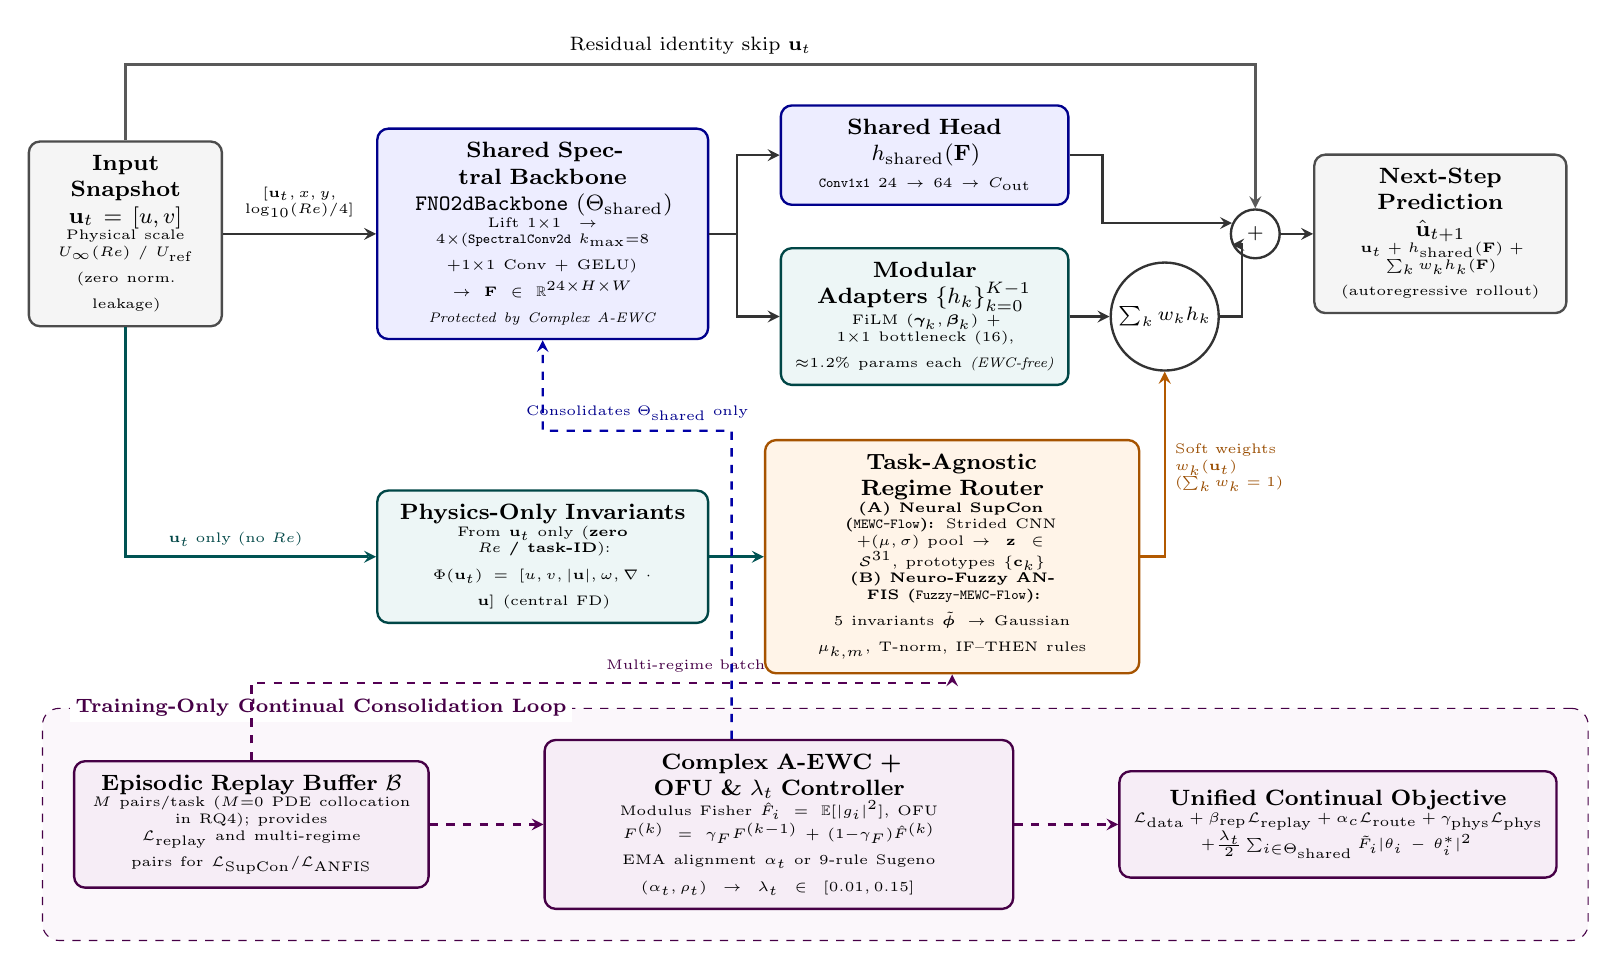
\begin{tikzpicture}[
    >=stealth,
    line width=0.85pt,
    font=\footnotesize,
    box/.style={draw=black!75, rounded corners=4pt, align=center, inner sep=5pt, minimum height=1.25cm},
    bluebox/.style={box, fill=blue!7, draw=blue!55!black},
    tealbox/.style={box, fill=teal!7, draw=teal!55!black},
    amberbox/.style={box, fill=orange!9, draw=orange!65!black},
    purplebox/.style={box, fill=violet!7, draw=violet!55!black},
    graybox/.style={box, fill=gray!8, draw=black!70},
    opcirc/.style={draw=black!80, circle, fill=white, align=center, inner sep=2pt, font=\scriptsize\bfseries},
    arr/.style={->, draw=black!80, line width=0.9pt},
    darr/.style={->, dashed, draw=black!75, line width=0.85pt}
  ]

  % --- Top Band: Shared Spectral Backbone + Modular Adapters ---
  \node[graybox, text width=2.1cm] (inp) at (0.85, 5.75) {%
    \textbf{Input Snapshot}\\
    $\mathbf{u}_t = [u, v]$\\
    {\tiny Physical scale $U_\infty(Re)$ / $U_{\text{ref}}$\\(zero norm.\ leakage)}%
  };

  \node[bluebox, text width=3.85cm] (fno) at (6.15, 5.75) {%
    \textbf{Shared Spectral Backbone}\\
    \texttt{FNO2dBackbone} ($\Theta_{\text{shared}}$)\\
    {\tiny Lift $1{\times}1 \to 4{\times}$(\texttt{SpectralConv2d} $k_{\max}{=}8$\\
    $+ 1{\times}1$ Conv + GELU) $\to \mathbf{F}\in\mathbb{R}^{24{\times}H{\times}W}$}\\
    {\tiny\itshape Protected by Complex A-EWC}%
  };

  \node[bluebox, text width=3.3cm, minimum height=1.05cm] (hshared) at (11.00, 6.75) {%
    \textbf{Shared Head} $h_{\text{shared}}(\mathbf{F})$\\
    {\tiny \texttt{Conv1x1} $24 \to 64 \to C_{\text{out}}$}%
  };

  \node[tealbox, text width=3.3cm, minimum height=1.15cm] (adapters) at (11.00, 4.70) {%
    \textbf{Modular Adapters} $\{h_k\}_{k=0}^{K-1}$\\
    {\tiny FiLM $(\boldsymbol{\gamma}_k,\boldsymbol{\beta}_k)$ + $1{\times}1$ bottleneck ($16$),\\
    ${\approx}1.2\%$ params each \textit{(EWC-free)}}%
  };

  \node[opcirc, minimum size=0.85cm] (mix) at (14.05, 4.70) {$\sum_k w_k h_k$};
  \node[opcirc, minimum size=0.62cm] (sumout) at (15.20, 5.75) {$+$};

  \node[graybox, text width=2.85cm] (out) at (17.55, 5.75) {%
    \textbf{Next-Step Prediction}\\
    $\hat{\mathbf{u}}_{t+1}$\\
    {\tiny $\mathbf{u}_t + h_{\text{shared}}(\mathbf{F}) + \sum_k w_k h_k(\mathbf{F})$\\
    (autoregressive rollout)}%
  };

  % Arrows in Top Band
  \draw[arr] (inp.east) -- node[above, align=center, font=\tiny, yshift=2pt] {$[\mathbf{u}_t, x, y,$\\$\log_{10}(Re)/4]$} (fno.west);
  \draw[arr] (fno.east) -- ++(0.35, 0) |- (hshared.west);
  \draw[arr] (fno.east) -- ++(0.35, 0) |- (adapters.west);
  \draw[arr] (adapters.east) -- (mix.west);
  \draw[arr] (hshared.east) -- ++(0.42, 0) |- (sumout.155);
  \draw[arr] (mix.east) -- ++(0.28, 0) |- (sumout.205);
  \draw[arr] (sumout.east) -- (out.west);

  % Residual skip connection
  \draw[arr, draw=black!65] (inp.north) -- (0.85, 7.90) -- node[above, font=\scriptsize] {Residual identity skip $\mathbf{u}_t$} (15.20, 7.90) -- (sumout.north);

  % --- Middle Band: Zero-Leakage Physics-Only Regime Routing ---
  \node[tealbox, text width=3.85cm, minimum height=1.2cm] (inv) at (6.15, 1.65) {%
    \textbf{Physics-Only Invariants}\\
    {\tiny From $\mathbf{u}_t$ only (\textbf{zero $Re$ / task-ID}):\\
    $\Phi(\mathbf{u}_t)=[u, v, |\mathbf{u}|, \omega, \nabla\cdot\mathbf{u}]$ (central FD)}%
  };

  \node[amberbox, text width=4.4cm, minimum height=1.45cm] (router) at (11.35, 1.65) {%
    \textbf{Task-Agnostic Regime Router}\\
    {\tiny \textbf{(A) Neural SupCon (\texttt{MEWC-Flow}):} Strided CNN\\
    $+ (\mu,\sigma)$ pool $\to \mathbf{z}\in\mathcal{S}^{31}$, prototypes $\{\mathbf{c}_k\}$\\
    \textbf{(B) Neuro-Fuzzy ANFIS (\texttt{Fuzzy-MEWC-Flow}):}\\
    5 invariants $\tilde{\boldsymbol{\phi}} \to$ Gaussian $\mu_{k,m}$, T-norm, IF--THEN rules}%
  };

  % Arrows in Middle Band
  \draw[arr, draw=teal!65!black] (inp.south) |- node[above, pos=0.72, font=\tiny, text=teal!55!black] {$\mathbf{u}_t$ only (no $Re$)} (inv.west);
  \draw[arr, draw=teal!65!black] (inv.east) -- (router.west);
  \draw[arr, draw=orange!70!black] (router.east) -| node[right, pos=0.74, align=left, font=\tiny, text=orange!60!black] {Soft weights\\$w_k(\mathbf{u}_t)$\\($\sum_k w_k=1$)} (mix.south);

  % --- Bottom Band: Training-Only Continual Consolidation Loop ---
  \node[purplebox, text width=4.15cm, minimum height=1.35cm] (replay) at (2.45, -1.75) {%
    \textbf{Episodic Replay Buffer} $\mathcal{B}$\\
    {\tiny $M$ pairs/task ($M{=}0$ PDE collocation\\
    in RQ4); provides $\mathcal{L}_{\text{replay}}$ and multi-regime\\
    pairs for $\mathcal{L}_{\text{SupCon}} / \mathcal{L}_{\text{ANFIS}}$}%
  };

  \node[purplebox, text width=5.6cm, minimum height=1.35cm] (aewc) at (9.15, -1.75) {%
    \textbf{Complex A-EWC + OFU \& $\lambda_t$ Controller}\\
    {\tiny Modulus Fisher $\hat{F}_i=\mathbb{E}[|g_i|^2]$, OFU $F^{(k)}=\gamma_F F^{(k-1)}+(1{-}\gamma_F)\hat{F}^{(k)}$\\
    EMA alignment $\alpha_t$ or 9-rule Sugeno $(\alpha_t,\rho_t)\to \lambda_t\in[0.01,0.15]$}%
  };

  \node[purplebox, text width=5.2cm, minimum height=1.35cm] (loss) at (16.25, -1.75) {%
    \textbf{Unified Continual Objective}\\
    {\tiny $\mathcal{L}_{\text{data}} + \beta_{\text{rep}}\mathcal{L}_{\text{replay}} + \alpha_c\mathcal{L}_{\text{route}} + \gamma_{\text{phys}}\mathcal{L}_{\text{phys}}$\\
    $+ \frac{\lambda_t}{2}\sum_{i\in\Theta_{\text{shared}}}\tilde{F}_i|\theta_i - \theta_i^*|^2$}%
  };

  \begin{scope}[on background layer]
    \node[draw=violet!55!black, dashed, rounded corners=6pt, fill=violet!3, fit=(replay) (aewc) (loss), inner sep=11pt, label={[font=\scriptsize\bfseries, text=violet!55!black, fill=white, inner sep=2pt, anchor=west, xshift=10pt]north west:{Training-Only Continual Consolidation Loop}}] (trainbox) {};
  \end{scope}

  % Arrows in Bottom Band (routed through open channels with zero crossings)
  \draw[darr, draw=violet!65!black] (replay.east) -- (aewc.west);
  \draw[darr, draw=violet!65!black] (aewc.east) -- (loss.west);
  \draw[darr, draw=violet!65!black] (replay.north) -- (2.45, 0.05) -- node[above, pos=0.62, font=\tiny, text=violet!55!black] {Multi-regime batch} (11.35, 0.05) -- (router.south);
  \draw[darr, draw=blue!65!black] ($(aewc.north)-(0.60,0)$) -- (8.55, 3.25) -- node[above, font=\tiny, text=blue!55!black] {Consolidates $\Theta_{\text{shared}}$ only} (6.15, 3.25) -- (fno.south);
\end{tikzpicture}%
}
\caption{End-to-end architecture of \textbf{MEWC-Flow} and neuro-fuzzy \textbf{Fuzzy-MEWC-Flow}. The shared spectral backbone (\texttt{FNO2dBackbone}, protected by complex-parameter A-EWC/OFU) extracts spatial features $\mathbf{F}$ and predicts base dynamics $h_{\text{shared}}(\mathbf{F})$, while lightweight FiLM + bottleneck adapters $\{h_k\}$ stay unconsolidated to learn regime-specific residual scales. At inference time, the router computes soft weights $w_k(\mathbf{u}_t)$ strictly from velocity invariants $\Phi(\mathbf{u}_t)$ (zero $Re$ or task-ID input), either via Supervised Contrastive prototypes (\texttt{MEWC-Flow}) or interpretable Gaussian ANFIS memberships and 9-rule Sugeno $\lambda_t$ control (\texttt{Fuzzy-MEWC-Flow}).}
\label{fig:architecture}
\end{figure}

\subsection{Shared Spectral Backbone}

For 2D benchmarks (\texttt{mewc\_flow/models/fno2d.py}), the shared backbone (\texttt{FNO2dBackbone}) takes the normalized velocity field concatenated with normalized spatial coordinates $(x, y)$ and a broadcast physical scaling channel (e.g., $\log_{10}(Re)/4$ when conditioned, passed as zero during strict unlabelled ablation checks), projects through a $1 \times 1$ lifting convolution to channel width $d_h = 24$, applies $L = 4$ residual blocks each combining a complex \texttt{SpectralConv2d} layer (retaining $k_{\max} = 8$ Fourier modes per axis) with a local $1 \times 1$ convolution and GELU activation, and outputs a base residual update $h_{\text{shared}}(\mathbf{F})$ ($299{,}186$ parameters in the base 2D model; $340{,}018$ parameters in full modular 2D MEWC-Flow). For 1D Burgers flow (\texttt{mewc\_flow/models/surrogate.py}), \texttt{FNO1d} uses $L = 3$ spectral blocks with $d_h = 32$ and $k_{\max} = 16$ modes ($54{,}625$ base / $76{,}065$ modular parameters). All models predict the temporal increment $\hat{\mathbf{u}}_{t+1} = \mathbf{u}_t + \Delta \hat{\mathbf{u}}$.

\subsection{Physics-Only Contrastive Regime Encoder \& Soft Routing (RQ3)}

To route adapters at inference time \textbf{without} privileged $Re$ or task-ID metadata, \texttt{PhysicsRegimeEncoder2d} computes purely flow-derived spatial differential invariants from the velocity input $\mathbf{u}_t = (u, v)$ alone:
\begin{equation}
\Phi(\mathbf{u}_t) = \left[u, \; v, \; \sqrt{u^2 + v^2 + \epsilon}, \; \omega = \frac{\partial v}{\partial x} - \frac{\partial u}{\partial y}, \; \delta = \frac{\partial u}{\partial x} + \frac{\partial v}{\partial y}\right] \in \mathbb{R}^{5 \times H \times W},
\end{equation}
computed via central finite differences (and $\Phi_{1\text{d}}(u_t) = [u, u_x, u_{xx}] \in \mathbb{R}^{3 \times N_x}$ in 1D). Zero Reynolds number or task-ID channel ever enters this encoder (verified by gradient and perturbation leakage tests in \texttt{tests/test\_verification.py}). A strided CNN pools both spatial means and standard deviations (capturing wake deficit alongside turbulent fluctuation energy and enstrophy) into an $L_2$-normalized hyperspherical embedding $\mathbf{z}(\mathbf{u}_t) \in \mathcal{S}^{d_z - 1}$ ($d_z = 32$).

When training task $k$ alongside replayed prior tasks $j < k$ (which supply multi-class negative and positive pairs in the mixed mini-batch), the encoder optimizes a Supervised Contrastive (SupCon) loss~\cite{khosla2020supcon} with temperature $\tau_c = 0.10$:
\begin{equation}
\mathcal{L}_{\text{SupCon}} = -\sum_{i \in I} \frac{1}{|P(i)|} \sum_{p \in P(i)} \log \frac{\exp(\mathbf{z}_i^{\top} \mathbf{z}_p / \tau_c)}{\sum_{a \in I \setminus \{i\}} \exp(\mathbf{z}_i^{\top} \mathbf{z}_a / \tau_c)},
\end{equation}
where $P(i)$ indexes samples sharing the regime identity of sample $i$ in the replay-augmented batch. After each stage, the normalized class prototype $\mathbf{c}_k = \text{norm}(\mathbb{E}_{\mathbf{u} \in \mathcal{D}_k}[\mathbf{z}(\mathbf{u})])$ is frozen. At inference time (task-agnostic), soft cosine attention blends active adapters:
\begin{equation}
w_k(\mathbf{u}_t) = \frac{\exp(\mathbf{z}(\mathbf{u}_t)^{\top} \mathbf{c}_k / \tau_{\text{route}})}{\sum_{m=0}^{K-1} \exp(\mathbf{z}(\mathbf{u}_t)^{\top} \mathbf{c}_m / \tau_{\text{route}})}, \qquad \hat{\mathbf{u}}_{t+1} = \mathbf{u}_t + h_{\text{shared}}(\mathbf{F}) + \sum_{k=0}^{K-1} w_k(\mathbf{u}_t)\, h_k(\mathbf{F}),
\end{equation}
allowing seamless interpolation for held-out intermediate Reynolds numbers (e.g., $Re = 910, 1890$). Hard top-1, uniform, and oracle routing modes are also supported for controlled ablation.

\subsection{Lightweight Modular Regime Adapters}

Each regime adapter \texttt{RegimeAdapter2d} ($k \in \{0, \dots, K-1\}$) acts on the backbone feature tensor $\mathbf{F} \in \mathbb{R}^{B \times 24 \times H \times W}$ via Feature-wise Linear Modulation ($\boldsymbol{\gamma}_k, \boldsymbol{\beta}_k$) followed by a $1 \times 1$ bottleneck residual block (width 16) outputting $h_k(\mathbf{F}) \in \mathbb{R}^{B \times C_{\text{out}} \times H \times W}$. Each adapter introduces only $\approx 1.2\%$ of the backbone parameters, remaining isolated from shared EWC penalties so regime-specific amplitude scales can adapt freely.

\subsection{Complex-Parameter Adaptive EWC (A-EWC) \& Online Fisher Updating}

Extending MEWC-RL++~\cite{hasan2026mewcrlpp} to complex Fourier spectral weights $\theta_i \in \mathbb{C}$, \texttt{mewc\_flow/models/ewc.py} defines the strictly real diagonal Fisher Information using complex gradient modulus squared and exact per-sample normalization:
\begin{equation}
\hat{F}_i^{(k)} = \frac{1}{N_{\text{seen}}} \sum_{n=1}^{N_{\text{seen}}} \left|\frac{\partial \ell_n}{\partial \theta_i}\right|^2, \qquad |g_i|^2 = \operatorname{Re}(g_i)^2 + \operatorname{Im}(g_i)^2.
\end{equation}
Rather than storing $K$ separate Fisher buffers, Online Fisher Updating (OFU) maintains $\mathcal{O}(|\theta_{\text{shared}}|)$ memory via exponential decay $\gamma_F = 0.85$:
\begin{equation}
F^{(k)} = \gamma_F F^{(k-1)} + (1 - \gamma_F)\hat{F}^{(k)}.
\end{equation}
To prevent scale collapse across datasets of widely differing MSE magnitudes (PIV $10^{-3}$ vs.\ ERA5 $2 \times 10^{-2}$ vs.\ Burgers $10^{-5}$), \texttt{AdaptiveEWC} applies empirical-Bayes scale normalization using stored task loss $\mathcal{L}_{\text{scale}}$ and natural step radius $r_0^2 = 10^{-6}$ over only the protected \textbf{shared backbone parameters} (\texttt{param\_allowlist}). At optimization step $t$, gradient memory tracking computes EMA alignment between current shared-parameter gradient $\mathbf{g}_t$ and running gradient memory $\mathbf{g}_{\text{prev}}^{(t)} = \beta_g \mathbf{g}_{\text{prev}}^{(t-1)} + (1 - \beta_g)\mathbf{g}_t$ ($\beta_g = 0.9$):
\begin{equation}
\alpha_t = \frac{\operatorname{Re}\langle \mathbf{g}_t, \mathbf{g}_{\text{prev}}^{(t-1)} \rangle}{\|\mathbf{g}_t\|_2 \, \|\mathbf{g}_{\text{prev}}^{(t-1)}\|_2 + \epsilon} \in [-1, 1], \qquad \lambda_t = \lambda_{\min} + \left(1 - \frac{1 + \alpha_t}{2}\right)(\lambda_{\max} - \lambda_{\min}),
\end{equation}
with $\lambda_{\min} = 0.01, \lambda_{\max} = 0.15$. Under gradient conflict ($\alpha_t < 0$), $\lambda_t \to \lambda_{\max}$ to stiffen critical shared modes; under aligned gradients ($\alpha_t > 0$), $\lambda_t \to \lambda_{\min}$ to permit forward transfer.

\subsection{Combined Objective, Replay \& Unified Optimization}

At task $k > 0$, MEWC-Flow minimizes:
\begin{equation}
\mathcal{L}_{\text{total}} = \mathcal{L}_{\text{data}}^{(k)} + \beta_{\text{rep}} \mathcal{L}_{\text{replay}} + \alpha_c \mathcal{L}_{\text{SupCon}} + \gamma_{\text{phys}} \mathcal{L}_{\text{phys}} + \frac{\lambda_t}{2} \sum_{i \in \Theta_{\text{shared}}} \tilde{F}_i \left|\theta_i - \theta_i^*\right|^2,
\end{equation}
with $\beta_{\text{rep}} = 1.0$, $\alpha_c = 0.25$ ($\tau_c = 0.10$), and $\gamma_{\text{phys}} = 0.05$ in 2D (penalizing both velocity divergence $\|\nabla \cdot \hat{\mathbf{u}}\|_2^2$ and finite-difference vorticity error $\|\hat{\omega} - \omega_{\text{true}}\|_2^2$) or $\gamma_{\text{phys}} = 0.02$ in 1D (viscous Burgers PDE residual). For the zero-data variant \texttt{MEWC-PDE-Replay} (RQ4), episodic storage is set strictly to $M = 0$ (\texttt{use\_replay=False}) while collocation perturbations from earlier viscosity parameters receive differentiable PDE-residual supervision (\texttt{burgers\_pde\_residual\_torch}). All baselines and MEWC-Flow share identical optimizer settings: \texttt{Adam} ($\text{lr} = 10^{-3}$), \texttt{CosineAnnealingLR} ($\eta_{\min} = 0.01 \cdot \text{lr}$), and gradient clipping at $\|\mathbf{g}\|_2 \le 1.0$.

\subsection{Neuro-Fuzzy Extension: \texttt{Fuzzy-MEWC-Flow} (\texttt{fuzzy\_logic.py})}

To replace opaque routing weights and purely linear $\lambda_t$ scheduling with human-interpretable physical rules~\cite{mamdani1974fuzzy,takagi1985fuzzy,jang1993anfis}, \textbf{\texttt{Fuzzy-MEWC-Flow}} introduces two principled neuro-fuzzy modules (\texttt{mewc\_flow/models/fuzzy\_logic.py}):
\begin{enumerate}
  \item \textbf{Takagi--Sugeno (ANFIS) Physical Regime Router (\texttt{TakagiSugenoRegimeRouter}):} Operates strictly on 5 scalar dimensionless flow invariants computed directly from $\mathbf{u}_t$ (zero $Re$ input) in 2D: kinetic energy $\text{KE}$, spatial turbulence kinetic variance $\text{TKE}_{\text{var}}$, $\log(1 + \text{Enstrophy})$, $\log(1 + \sigma_{\omega})$, and $\log(1 + \|\nabla\cdot\mathbf{u}\|_2^2)$ (and 4 shock/curvature invariants $[u^2, \log(1+u_x^2), \log(1+\max|u_x|), \log(1+u_{xx}^2)]$ in 1D). Feature standardization $(\mu_0, \sigma_0)$ is fitted strictly on Task-0 (zero future-regime leakage). Each regime $k$ learns a multi-dimensional Gaussian membership function $\mu_{k,m}(\tilde{\phi}_m) = \exp(-(\tilde{\phi}_m - c_{k,m})^2 / (2\sigma_{k,m}^2))$ ($\sigma_{k,m} \ge 0.20$), combined via log-space product T-norm and softmax normalization ($\tau_{\text{fuzzy}} = 1.0$) into partition-of-unity adapter weights $\bar{w}_k(\mathbf{u}_t)$ sharpened end-to-end on replay-mixed batches.
  \item \textbf{9-Rule Zero-Order Sugeno Stability--Plasticity Controller (\texttt{FuzzyAdaptiveEWC}):} Maps EMA gradient cosine alignment $\alpha_t \in [-1, 1]$ (\texttt{Conflict = -1, Neutral = 0, Aligned = +1}, $\sigma_{\alpha} = 0.55$) and normalized EMA loss drift $\rho_t = \tanh(2(\mathcal{L}_t - \bar{\mathcal{L}}) / \bar{\mathcal{L}}) \in [-1, 1]$ (\texttt{LowDrift = -0.6, ModDrift = 0.0, HighDrift = +0.6}, $\sigma_{\rho} = 0.45$) through a $3 \times 3$ zero-order Sugeno consequent table $U = [[0.65, 0.85, 1.00], [0.25, 0.45, 0.75], [0.00, 0.15, 0.40]]$ via centroid defuzzification into $\lambda_t \in [\lambda_{\min}, \lambda_{\max}]$.
\end{enumerate}

\begin{algorithm}[!htbp]
\caption{MEWC-Flow Continual Learning \& Task-Agnostic Inference}
\label{alg:mewcflow}
\begin{algorithmic}[1]
\REQUIRE Sequential tasks $\{\mathcal{D}_k^{\text{train}}\}_{k=0}^{K-1}$, shared FNO backbone $\Theta_{\text{shared}}$, adapters $\{h_k\}_{k=0}^{K-1}$, physics-only encoder $e_{\psi}$, episodic buffer $\mathcal{B}$ (cap $M$ per task), bounds $[\lambda_{\min}, \lambda_{\max}]$.
\STATE Initialize $\mathbf{g}_{\text{prev}} \gets \mathbf{0}$, $\mathcal{B} \gets \emptyset$, consolidated flag $\gets \text{False}$.
\FOR{$k = 0, \dots, K-1$}
  \STATE Initialize Adam ($\text{lr}=10^{-3}$) + CosineAnnealingLR ($\eta_{\min}=10^{-5}$) over active parameters.
  \FOR{each mini-batch $(\mathbf{u}_t, \mathbf{u}_{t+1}) \sim \mathcal{D}_k^{\text{train}}$}
    \STATE Compute task loss $\mathcal{L}_{\text{data}}^{(k)}$ and physical regularization $\mathcal{L}_{\text{phys}}$ (vorticity + divergence / PDE residual).
    \IF{$k > 0$ and $|\mathcal{B}| > 0$}
      \STATE Sample replay batch $(\mathbf{u}_r, \mathbf{u}_{r+1}, y_r) \sim \mathcal{B}$; compute $\mathcal{L}_{\text{replay}}$ and $\mathcal{L}_{\text{SupCon}}$ on $\Phi(\mathbf{u})$.
      \STATE Compute shared-backbone gradient alignment $\alpha_t$ against $\mathbf{g}_{\text{prev}}$ and dynamic $\lambda_t \in [\lambda_{\min}, \lambda_{\max}]$.
      \STATE Evaluate Complex A-EWC quadratic penalty $\frac{\lambda_t}{2}\sum_{i\in\Theta_{\text{shared}}} \tilde{F}_i |\theta_i - \theta_i^*|^2$.
    \ENDIF
    \STATE Update weights with $\|\mathbf{g}\|_2 \le 1.0$ clipping; update EMA gradient memory $\mathbf{g}_{\text{prev}}$.
  \ENDFOR
  \STATE Freeze normalized contrastive prototype $\mathbf{c}_k \gets \text{norm}(\mathbb{E}_{\mathbf{u}\in\mathcal{D}_k}[e_{\psi}(\Phi(\mathbf{u}))])$.
  \STATE Store $M$ exemplars from $\mathcal{D}_k^{\text{train}}$ into $\mathcal{B}$.
  \STATE Estimate complex diagonal Fisher $\hat{F}^{(k)}$ on $\Theta_{\text{shared}}$ and apply Online Fisher Updating: $F^{(k)} \gets \gamma_F F^{(k-1)} + (1-\gamma_F)\hat{F}^{(k)}$.
\ENDFOR
\STATE \textbf{Task-Agnostic Inference on Unseen $\mathbf{u}_t$:} Compute $\mathbf{z} \gets e_{\psi}(\Phi(\mathbf{u}_t))$ (zero $Re$ input), soft weights $w_k \gets \text{softmax}(\mathbf{z}^{\top}\mathbf{c}_k/\tau_{\text{route}})$, and predict $\hat{\mathbf{u}}_{t+1} = \mathbf{u}_t + h_{\text{shared}}(\mathbf{F}) + \sum_k w_k h_k(\mathbf{F})$.
\end{algorithmic}
\end{algorithm}

% ==============================================================================
\section{Experimental Setup \& Verification}
% ==============================================================================

\subsection{Four Continual Fluid Benchmarks}

\begin{enumerate}
  \item \textbf{Benchmark 1: Laboratory PIV Cylinder Wakes (\texttt{Caltech PIV}~\cite{renn2026piv}).} Real planar velocity measurements $(u, v)$ on a $64 \times 64$ spatial grid across four sequential sub-critical Reynolds regimes: $Re = 240 \to 650 \to 1280 \to 2520$, with held-out intermediate regimes $Re = 910, 1890$. Trained for 15 epochs/task across 5 seeds (\texttt{42, 102, 202, 302, 402}), episodic buffer $M = 16$ exemplars/task. Run boundaries ($t \bmod 100$) are strictly respected.
  \item \textbf{Benchmark 2: 2D Kolmogorov Navier--Stokes Bifurcation.} High-order pseudo-spectral RK4 simulation of incompressible 2D Navier--Stokes on $[0, 2\pi]^2$ ($64 \times 64$) with Kolmogorov forcing $f(y) = \sin(4y)$ across a tenfold bifurcation jump: $Re = 20$ (steady laminar) $\to Re = 45$ (supercritical instability onset) $\to Re = 120$ (transitional vortex shedding) $\to Re = 400$ (chaotic 2D turbulence), with held-out $Re = 75, 240$. Trained 12 epochs/task across 3 seeds (\texttt{42, 102, 202}), $M = 16$. Exact vorticity transport PDE residual and divergence are evaluated on predicted fields.
  \item \textbf{Benchmark 3: ERA5 Global 10-m Planetary Winds (\texttt{WeatherBench 2}~\cite{rasp2024wb2}).} Real 6-hourly global horizontal winds $(u_{10}, v_{10})$ ($64 \times 64$ grid, normalized by $U_{\text{ref}} = 10.0\text{ m/s}$) across four chronological 2020 seasonal tasks (\texttt{Winter -> Spring -> Summer -> Autumn}), evaluated additionally on full chronological held-out \texttt{Summer 2019} and \texttt{Winter 2019} (123 transitions each) and 72-h (12-step) autoregressive rollouts plus Northern Hemisphere storm-track spatial slice RMSE. Trained 18 epochs/task across 3 seeds (\texttt{42, 102, 202}), $M = 16$.
  \item \textbf{Benchmark 4: 1D Viscous Burgers Shock Formation \& RQ4.} Periodic 1D Burgers flow ($N_x = 128$, $N_t = 40$) spanning a $100\times$ viscosity drop $\nu = 0.05 \to 0.01 \to 0.002 \to 0.0005$ (held-out $\nu = 0.02, 0.005$), trained 20 epochs/task across 3 seeds (\texttt{42, 102, 202}), $M = 32$. Includes a capacity-constrained stress test (\texttt{width=16}, \texttt{modes=12}, 25 epochs/task).
\end{enumerate}

\subsection{Baselines, Memory Accounting \& Verification Protocol}

We compare against \texttt{Fine-Tuning} (lower bound), \texttt{EWC} (additive diagonal complex Fisher, $\lambda = 2.0$), \texttt{Online-EWC} ($\gamma_F = 0.85, \lambda = 2.0$), \texttt{ER}~\cite{rolnick2019er} (reservoir episodic replay), \texttt{Replay-TS}~\cite{hemati2026replayts} (temporal-slicing replay), \texttt{SLE-FNO}~\cite{elhadidy2026slefno} (single-layer extensions on frozen backbone), \texttt{MEWC-PDE-Replay} (zero-data PDE replay on Burgers), and offline \texttt{Joint} training (upper bound). Extra CL memory (\texttt{Extra MB}) is computed directly from exact buffer, adapter, Fisher, $\theta^*$, and encoder byte sizes (\texttt{mewc\_flow/utils/results\_io.py}). Every claim and table is programmatically cross-checked via \texttt{tests/test\_verification.py} and \texttt{tests/verify\_manuscript\_numbers.py} with strict JSON (\texttt{allow\_nan=False}), paired two-sided $t$-tests, and Cohen's $d$.

% ==============================================================================
\section{Error Analysis Process \& Experimental Findings}
% ==============================================================================

\subsection{Six-Layer Error Analysis Process}

Because single-step pixel MSE fails to detect physical drift, unphysical divergence, or non-stationary breakdown in fluid surrogates, we engineered a systematic \textbf{six-layer error analysis process} implemented across \texttt{mewc\_flow/utils/metrics.py}, \texttt{physics\_metrics.py}, \texttt{stats.py}, and \texttt{piv\_experiments/}:

\begin{enumerate}
  \item \textbf{Continual Retention \& Transfer Matrix Tracking:} Recording the complete lower-triangular evaluation matrix $E_{i,j}$ after every task $i$ to isolate catastrophic forgetting ($-\text{BWT}$), Task-0 relative degradation (\%), and zero-shot held-out interpolation MSE on intermediate Reynolds numbers and held-out atmospheric years.
  \item \textbf{Multi-Window Autoregressive Rollouts \& Valid Prediction Horizon:} Evaluating recursive rollout relative-$L_2$ drift across $t \in [1, 20]$ steps (2D PIV, Kolmogorov NS, 1D Burgers) and 72-h ($12 \times 6\text{h}$) weather rollouts (ERA5), alongside $\text{VPH}_{0.25}$ (earliest step where relative $L_2$ exceeds $0.25$).
  \item \textbf{Physical Invariant, PDE Residual \& Spectral Band Decomposition:} Auditing finite-difference vorticity RMSE, divergence RMSE ($\|\nabla \cdot \mathbf{u}\|_{\text{RMS}}$), exact 2D Kolmogorov Navier--Stokes vorticity-transport PDE residual and 1D Burgers PDE residual, kinetic energy/enstrophy relative errors, and radial 2D energy spectra $E(k)$ decomposed into low-, mid- (inertial), and high-wavenumber bands (\texttt{physics\_and\_rollout\_summary.json}).
  \item \textbf{Zero-Leakage Latent Manifold \& Routing Failure Audit:} Projecting physics-only encoder embeddings $\mathbf{z}(\mathbf{u}_t)$ via PCA, measuring cluster silhouette scores and nearest-prototype confusion matrices without $Re$ supervision, and inspecting soft routing weight matrices across both seen and held-out Reynolds numbers (\texttt{latent\_manifold\_summary.json}).
  \item \textbf{Component Ablation, Curriculum Ordering \& Byte-Level Memory Pareto Sweeps:} Systematically ablating each architectural and loss component (8 variants), routing mechanism (soft, hard, uniform, oracle), task ordering (ascending, descending, shuffled), and replay capacity $M \in \{4, 8, 16, 32\}$ (\texttt{ablation\_study\_summary.json}), alongside a capacity-bottlenecked stress test on Burgers (\texttt{width=16}).
  \item \textbf{Matched-Seed Statistical Significance \& Strict-JSON Integrity:} Computing two-sided paired $t$-tests ($p$-values) and Cohen's $d$ effect sizes across identical random seeds against every baseline, enforced via strict JSON (\texttt{allow\_nan=False}) and \texttt{tests/verify\_manuscript\_numbers.py}.
\end{enumerate}

\subsection{Main PIV Cylinder Wake Benchmark (RQ1 \& RQ2)}

\begin{table}[!htbp]
\centering
\caption{Caltech PIV cylinder wake benchmark ($Re = 240 \to 650 \to 1280 \to 2520$, 5 seeds, 15 epochs/task, $M = 16$). Significance markers compare each baseline against MEWC-Flow ($^{*}p < 0.05$, $^{**}p < 0.01$, paired two-sided $t$-test across matched seeds). Lower is better for all metrics; negative forgetting denotes positive backward transfer.}
\label{tab:piv_main}
\resizebox{\textwidth}{!}{%
\begin{tabular}{@{}lcccccc@{}}
\toprule
Method & Avg.\ Forgetting ($\Delta$MSE) & Final MSE (4 regimes) & $Re=240$ Rollout Rel-$L_2$ ($t=10$) & $Re=240$ Vorticity RMSE & Held-out MSE ($Re=910, 1890$) & Extra Memory (MB) \\
\midrule
Fine-Tuning & $4.34 \times 10^{-4} \pm 4.1 \times 10^{-4}$$^{*}$ & $1.43 \times 10^{-3} \pm 3.1 \times 10^{-4}$$^{*}$ & $0.2125 \pm 0.0633$$^{*}$ & $0.0358 \pm 0.0057$ & $1.51 \times 10^{-3} \pm 1.9 \times 10^{-4}$$^{*}$ & 0.00 \\
EWC & $-2.25 \times 10^{-5} \pm 5.0 \times 10^{-6}$$^{**}$ & $1.26 \times 10^{-3} \pm 9.1 \times 10^{-6}$$^{**}$ & $0.1059 \pm 0.0053$ & $0.0280 \pm 0.0007$ & $1.50 \times 10^{-3} \pm 1.3 \times 10^{-5}$$^{**}$ & 3.57 \\
Online-EWC & $-1.09 \times 10^{-5} \pm 2.6 \times 10^{-5}$$^{**}$ & $1.24 \times 10^{-3} \pm 1.8 \times 10^{-5}$$^{**}$ & $0.1230 \pm 0.0237$ & $0.0289 \pm 0.0015$ & $1.47 \times 10^{-3} \pm 1.7 \times 10^{-5}$$^{**}$ & 3.57 \\
ER & $-8.02 \times 10^{-5} \pm 9.6 \times 10^{-6}$ & $1.03 \times 10^{-3} \pm 1.2 \times 10^{-5}$$^{*}$ & $0.0997 \pm 0.0043$ & $0.0279 \pm 0.0017$ & $1.26 \times 10^{-3} \pm 1.0 \times 10^{-5}$$^{*}$ & 4.20 \\
Replay-TS & $-7.94 \times 10^{-5} \pm 9.7 \times 10^{-6}$ & $1.06 \times 10^{-3} \pm 1.6 \times 10^{-5}$$^{**}$ & $0.0981 \pm 0.0019$ & $0.0270 \pm 0.0012$ & $1.29 \times 10^{-3} \pm 1.9 \times 10^{-5}$ & 3.93 \\
SLE-FNO & $2.60 \times 10^{-7} \pm 2.8 \times 10^{-7}$$^{**}$ & $1.34 \times 10^{-3} \pm 6.0 \times 10^{-6}$$^{**}$ & $0.1237 \pm 0.0029$$^{**}$ & $0.0320 \pm 0.0006$$^{*}$ & $1.59 \times 10^{-3} \pm 5.7 \times 10^{-6}$$^{**}$ & 0.01 \\
\textbf{MEWC-Flow} & $\mathbf{-7.78 \times 10^{-5} \pm 1.8 \times 10^{-5}}$ & $\mathbf{1.05 \times 10^{-3} \pm 1.7 \times 10^{-5}}$ & $\mathbf{0.0997 \pm 0.0053}$ & $\mathbf{0.0278 \pm 0.0020}$ & $\mathbf{1.28 \times 10^{-3} \pm 2.1 \times 10^{-5}}$ & \textbf{10.32} \\
Joint & $0.00 \times 10^{0} \pm 0.0 \times 10^{0}$$^{**}$ & $1.05 \times 10^{-3} \pm 4.3 \times 10^{-5}$ & $0.0853 \pm 0.0043$$^{**}$ & $0.0242 \pm 0.0015$$^{*}$ & $1.28 \times 10^{-3} \pm 5.0 \times 10^{-5}$ & 38.80 \\
\bottomrule
\end{tabular}%
}
\end{table}

\begin{table}[!htbp]
\centering
\caption{Paired two-sided $t$-tests and Cohen's $d$ on Caltech PIV (MEWC-Flow minus baseline across 5 seeds). Negative $\Delta$ and $d < 0$ favor MEWC-Flow.}
\label{tab:piv_stats}
\resizebox{\textwidth}{!}{%
\begin{tabular}{@{}lccccc@{}}
\toprule
Comparison & $\Delta$Final MSE ($p$) & $\Delta$Forgetting ($p$) & $\Delta$Rollout $t=10$ ($p$) & $\Delta$Held-out MSE ($p$) & Cohen's $d$ (Final MSE) \\
\midrule
MEWC-Flow vs.\ Fine-Tuning & $-3.80 \times 10^{-4}$ (0.047) & $-5.12 \times 10^{-4}$ (0.045) & $-0.1127$ (0.020) & $-2.26 \times 10^{-4}$ (0.043) & $-1.27$ \\
MEWC-Flow vs.\ EWC & $-2.11 \times 10^{-4}$ (0.000) & $-5.52 \times 10^{-5}$ (0.001) & $-0.0061$ (0.228) & $-2.20 \times 10^{-4}$ (0.000) & $-13.97$ \\
MEWC-Flow vs.\ Online-EWC & $-1.93 \times 10^{-4}$ (0.000) & $-6.69 \times 10^{-5}$ (0.002) & $-0.0233$ (0.135) & $-1.89 \times 10^{-4}$ (0.000) & $-12.38$ \\
MEWC-Flow vs.\ ER & $+1.34 \times 10^{-5}$ (0.015) & $+2.41 \times 10^{-6}$ (0.745) & $-0.0000$ (0.996) & $+2.12 \times 10^{-5}$ (0.033) & $+1.84$ \\
MEWC-Flow vs.\ Replay-TS & $-1.49 \times 10^{-5}$ (0.002) & $+1.60 \times 10^{-6}$ (0.811) & $+0.0016$ (0.400) & $-6.56 \times 10^{-6}$ (0.398) & $-3.02$ \\
MEWC-Flow vs.\ SLE-FNO & $-2.94 \times 10^{-4}$ (0.000) & $-7.80 \times 10^{-5}$ (0.001) & $-0.0240$ (0.001) & $-3.13 \times 10^{-4}$ (0.000) & $-14.93$ \\
MEWC-Flow vs.\ Joint & $-5.71 \times 10^{-6}$ (0.731) & $-7.78 \times 10^{-5}$ (0.001) & $+0.0144$ (0.010) & $+2.02 \times 10^{-6}$ (0.916) & $-0.17$ \\
\bottomrule
\end{tabular}%
}
\end{table}

Sequential Fine-Tuning suffers $+134.8\%$ Task-0 relative degradation and drops to a valid prediction horizon ($\text{VPH}_{0.25}$) of only $14.3 \pm 5.6$ steps (vs.\ $20.0 \pm 0.0$ for all regularized/replay methods and MEWC-Flow), losing shear-layer phase coherence by $t=10$ (step-10 rel-$L_2 = 0.2125$; Table~\ref{tab:piv_main}). MEWC-Flow reduces Final MSE to $1.05 \times 10^{-3}$, making it statistically indistinguishable from full offline Joint training ($1.05 \times 10^{-3}$, $p = 0.731$; Table~\ref{tab:piv_stats}) while using $3.76\times$ less extra storage ($10.32\text{ MB}$ vs.\ $38.80\text{ MB}$) and beating EWC ($p < 10^{-4}$, $d = -13.97$), Online-EWC ($p < 10^{-4}$, $d = -12.38$), Replay-TS ($p = 0.002$, $d = -3.02$), and SLE-FNO ($p < 10^{-4}$, $d = -14.93$). Notice also the honest trade-off against monolithic \texttt{ER}: \texttt{ER} achieves slightly lower single-step Final MSE ($1.03 \times 10^{-3}$ vs.\ $1.05 \times 10^{-3}$, $p = 0.015$) at lower memory ($4.20\text{ MB}$), while matching MEWC-Flow on 10-step rollout ($0.0997$, $p = 0.996$). In seed-0 spectral diagnostics (\texttt{physics\_and\_rollout\_summary.json}, Fig.~\ref{fig:piv_physics}), however, MEWC-Flow exhibits the lowest \textbf{mid-wavenumber inertial-band log-spectral RMSE} ($0.0484$ vs.\ ER $0.0794$, Replay-TS $0.0817$, SLE-FNO $0.1057$, Fine-Tuning $0.3287$) and lowest seed-0 step-10 rollout rel-$L_2$ ($0.0927$) and vorticity RMSE ($0.0251$).

\begin{figure}[!htbp]
\centering
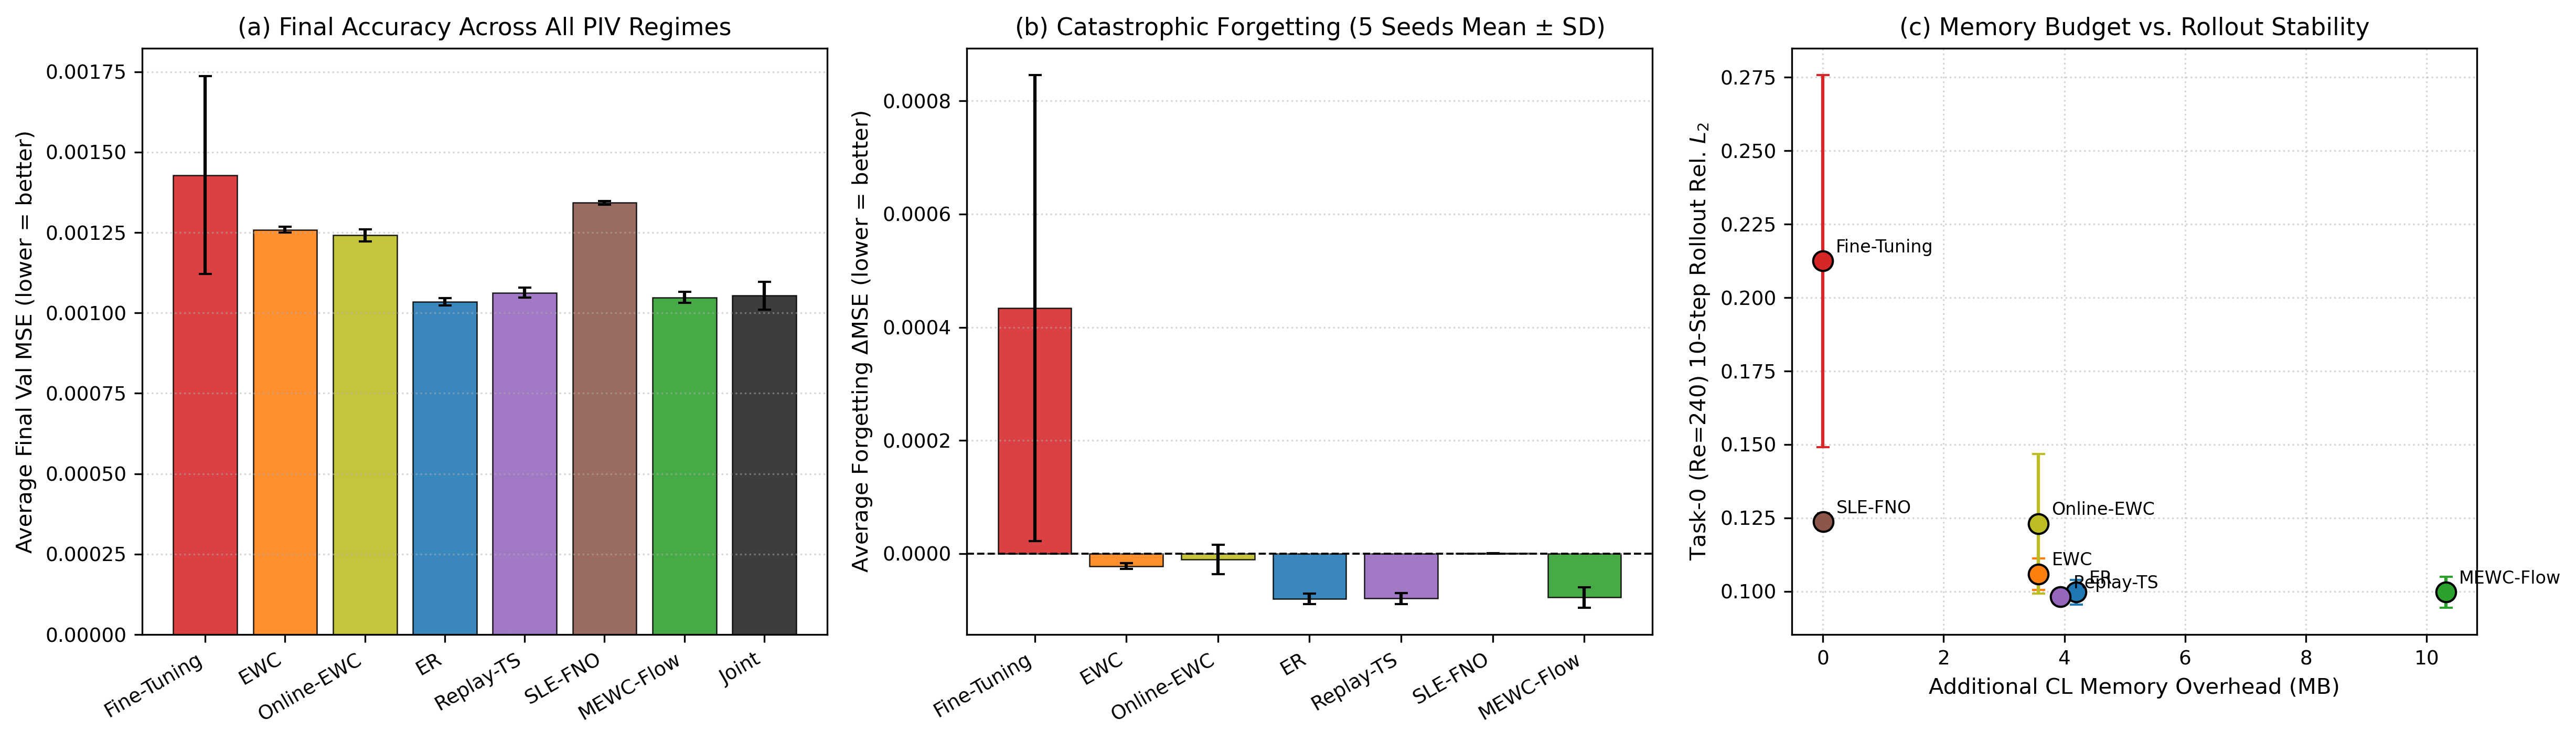
\includegraphics[width=0.96\textwidth,height=0.39\textheight,keepaspectratio]{mewc_flow/experiments/piv_experiments/results/fig1_piv_benchmark_and_forgetting.png}
\caption{PIV continual learning benchmark across 5 random seeds ($M=16$, 15 epochs/task): final MSE, catastrophic forgetting ($\Delta$MSE), Task-0 degradation, and held-out cross-$Re$ generalization.}
\label{fig:piv_main}
\end{figure}

\begin{figure}[!htbp]
\centering
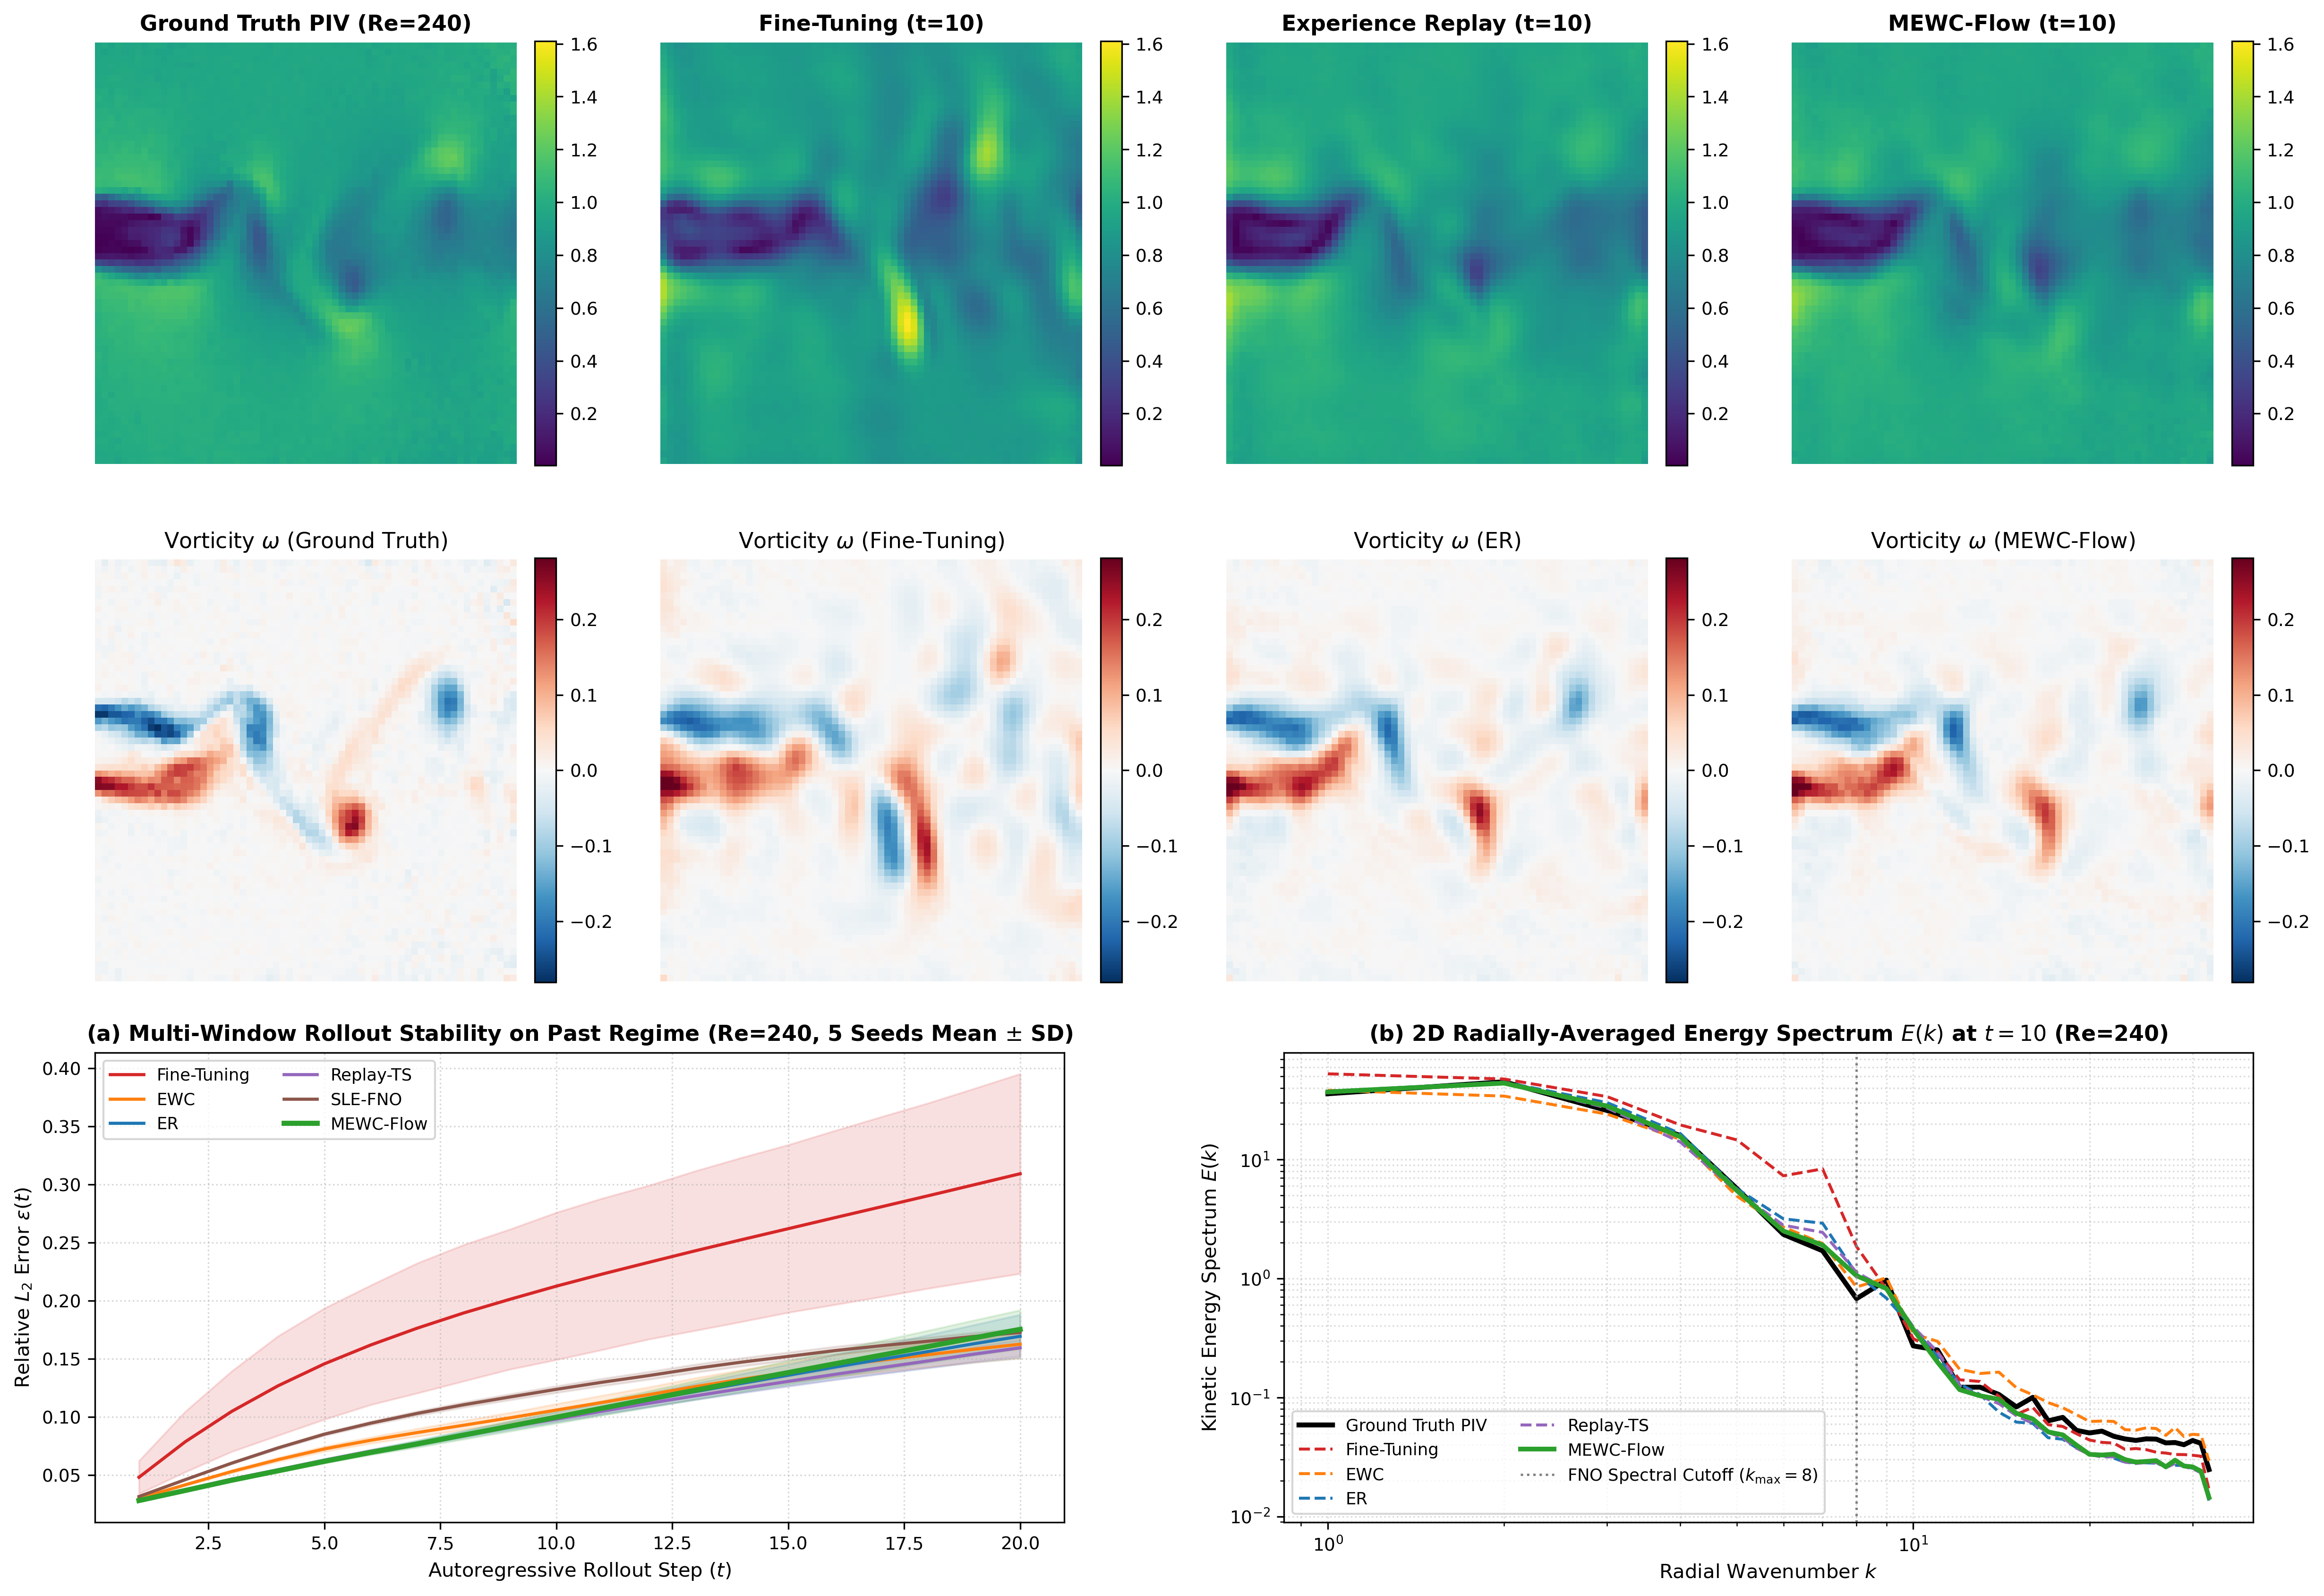
\includegraphics[width=0.96\textwidth,height=0.39\textheight,keepaspectratio]{mewc_flow/experiments/piv_experiments/results/fig2_piv_physics_rollout_spectrum.png}
\caption{Physical and spectral diagnostics on $Re=240$ after learning up to $Re=2520$: vorticity snapshots, divergence RMSE, kinetic energy spectra $E(k)$ highlighting MEWC-Flow's inertial-band accuracy, and multi-step autoregressive rollout drift.}
\label{fig:piv_physics}
\end{figure}

\FloatBarrier
\subsection{Zero-Leakage Physics-Only Regime Identification \& Routing (RQ3)}

Across all 5 PIV seeds, MEWC-Flow's physics-only contrastive encoder (\texttt{PhysicsRegimeEncoder2d}, zero $Re$ input) achieves $\mathbf{77.55\% \pm 4.61\%}$ task-agnostic regime classification accuracy and $\mathbf{0.4647 \pm 0.0560}$ latent silhouette score. On the representative seed-0 model (\texttt{latent\_manifold\_summary.json}, Fig.~\ref{fig:piv_latent}), nearest-prototype accuracy reaches $\mathbf{84.2\%}$ (silhouette $0.518$, first two PCA axes explaining $78.3\%$ and $18.4\%$ variance). The confusion matrix across the 196 test samples ($49$ per regime) is $\text{diag}/$block: $[[49, 0, 0, 0], [0, 18, 31, 0], [0, 0, 49, 0], [0, 0, 0, 49]]$: laminar ($Re=240$), transitional ($Re=1280$), and turbulent ($Re=2520$) regimes are $100\%$ separable purely from flow invariants, while all 31 misclassifications occur between adjacent transition wakes ($Re=650 \leftrightarrow 1280$) whose Strouhal shedding statistics overlap physically.

\begin{table}[!htbp]
\centering
\caption{Soft routing attention weights $w_k(\mathbf{u}_t)$ produced by the seed-0 MEWC-Flow encoder without $Re$ input ($^*$ denotes zero-shot unseen held-out Reynolds regimes).}
\label{tab:routing_weights}
\begin{tabular}{@{}lcccc@{}}
\toprule
Input Regime & Adapter $Re=240$ & Adapter $Re=650$ & Adapter $Re=1280$ & Adapter $Re=2520$ \\
\midrule
$Re=240$ & \textbf{0.97} & 0.03 & 0.00 & 0.00 \\
$Re=650$ & 0.00 & \textbf{0.64} & 0.36 & 0.00 \\
$Re=910^*$ & 0.00 & 0.07 & \textbf{0.92} & 0.00 \\
$Re=1280$ & 0.00 & 0.02 & \textbf{0.98} & 0.00 \\
$Re=1890^*$ & 0.00 & 0.00 & 0.04 & \textbf{0.96} \\
$Re=2520$ & 0.00 & 0.00 & 0.00 & \textbf{1.00} \\
\bottomrule
\end{tabular}
\end{table}

Notably, on unseen held-out regimes $Re=910^*$ and $Re=1890^*$ (Table~\ref{tab:routing_weights}), soft attention automatically interpolates neighboring high-Reynolds experts ($0.07 \cdot h_{650} + 0.92 \cdot h_{1280}$ and $0.04 \cdot h_{1280} + 0.96 \cdot h_{2520}$, respectively) purely from instantaneous flow invariants.

\begin{figure}[!htbp]
\centering
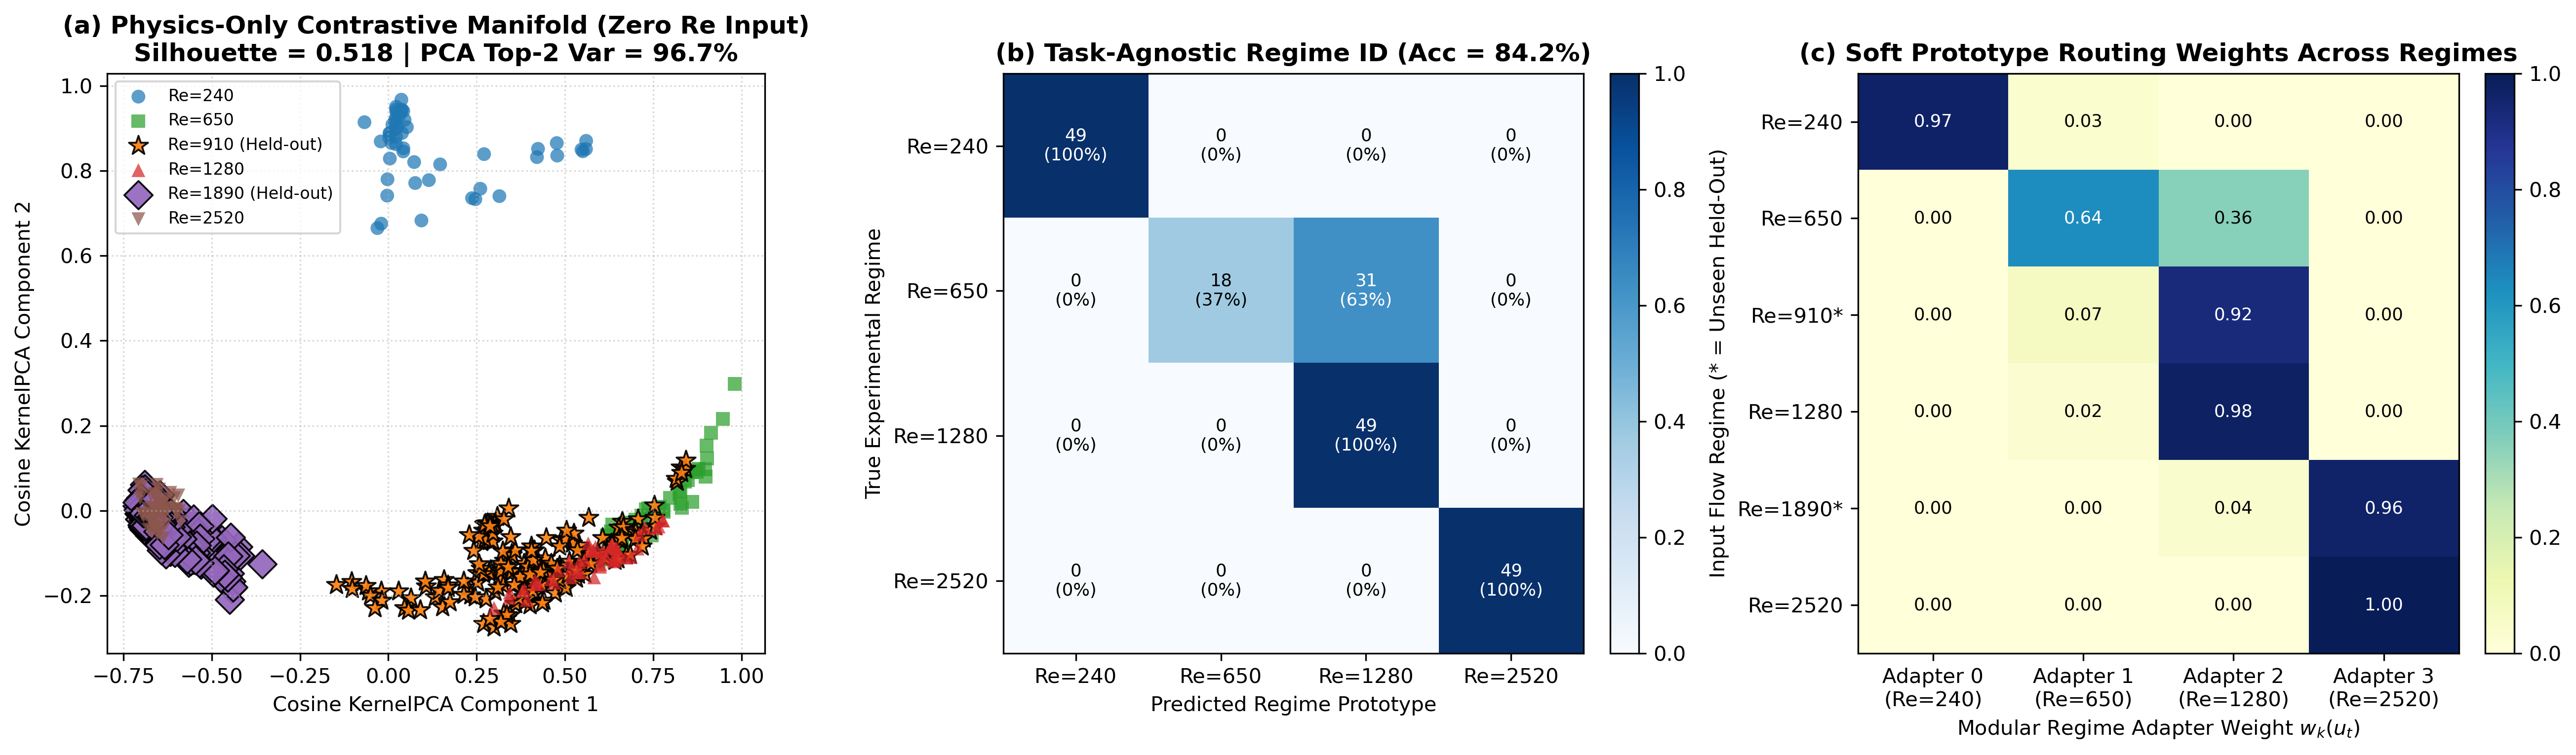
\includegraphics[width=0.96\textwidth,height=0.39\textheight,keepaspectratio]{mewc_flow/experiments/piv_experiments/results/fig3_piv_latent_manifold_and_routing.png}
\caption{Hyperspherical PCA projection of the physics-only contrastive latent space (left) and emergent diagonal/interpolated soft routing weights across seen and unseen Reynolds numbers (right).}
\label{fig:piv_latent}
\end{figure}

\FloatBarrier
\subsection{Component Ablations, Routing Modes, Task Ordering \& Memory Scaling (RQ1, RQ3, RQ5)}

Tables~\ref{tab:ablation}--\ref{tab:memory} report the 3-seed (\texttt{42, 102, 202}, 12 epochs/task) systematic PIV ablation suite. Removing episodic replay (\texttt{w/o Episodic Replay (0 MB)}) immediately collapses performance: forgetting jumps from $-9.80 \times 10^{-5}$ to $+4.28 \times 10^{-4}$, Final MSE degrades from $1.08 \times 10^{-3}$ to $1.50 \times 10^{-3}$, and Task-0 step-10 rollout error more than doubles from $0.0985 \pm 0.0043$ to $0.2248 \pm 0.0763$. This establishes \textbf{episodic replay as the primary anti-forgetting driver} on stationary-geometry PIV wakes. Equally informative is the tight clustering ($0.0953$--$0.0987$ step-10 rollout error) across all replay-equipped ablations on PIV: because cylinder geometry stays fixed across PIV tasks, lightweight adapters, contrastive routing, and EWC neither significantly degrade nor dramatically exceed raw \texttt{ER} on single-step PIV MSE. Instead, they provide interpretable regime-routing structure and Fisher consolidation needed when topology bifurcates (Section~\ref{sec:kolmogorov}) or dynamics shift seasonally (Section~\ref{sec:era5}).

\begin{table}[!htbp]
\centering
\caption{Systematic PIV component ablation across 3 seeds (\texttt{42, 102, 202}, 12 epochs/task).}
\label{tab:ablation}
\resizebox{\textwidth}{!}{%
\begin{tabular}{@{}lcccccc@{}}
\toprule
Variant & Avg.\ Forgetting & Final MSE & Rollout $t=10$ & Vorticity RMSE & Held-out MSE & Extra MB \\
\midrule
Full MEWC-Flow & $-9.80 \times 10^{-5} \pm 1.3 \times 10^{-5}$ & $1.08 \times 10^{-3} \pm 8.3 \times 10^{-6}$ & $0.0985 \pm 0.0043$ & $0.0273 \pm 0.0021$ & $1.31 \times 10^{-3} \pm 1.6 \times 10^{-5}$ & 10.32 \\
w/o Modular Adapters & $-1.14 \times 10^{-4} \pm 1.1 \times 10^{-5}$ & $1.06 \times 10^{-3} \pm 4.6 \times 10^{-6}$ & $0.0961 \pm 0.0026$ & $0.0263 \pm 0.0014$ & $1.28 \times 10^{-3} \pm 5.4 \times 10^{-6}$ & 10.31 \\
w/o Contrastive Router & $-9.83 \times 10^{-5} \pm 8.2 \times 10^{-6}$ & $1.09 \times 10^{-3} \pm 5.7 \times 10^{-6}$ & $0.0965 \pm 0.0036$ & $0.0265 \pm 0.0017$ & $1.31 \times 10^{-3} \pm 1.2 \times 10^{-5}$ & 10.15 \\
w/o Adaptive EWC (Static) & $-9.54 \times 10^{-5} \pm 9.3 \times 10^{-6}$ & $1.10 \times 10^{-3} \pm 2.9 \times 10^{-6}$ & $0.0976 \pm 0.0039$ & $0.0268 \pm 0.0018$ & $1.33 \times 10^{-3} \pm 1.1 \times 10^{-5}$ & 7.94 \\
w/o EWC & $-9.38 \times 10^{-5} \pm 1.4 \times 10^{-5}$ & $1.07 \times 10^{-3} \pm 1.1 \times 10^{-5}$ & $0.0987 \pm 0.0042$ & $0.0274 \pm 0.0019$ & $1.30 \times 10^{-3} \pm 1.7 \times 10^{-5}$ & 4.37 \\
w/o Episodic Replay (0 MB) & $+4.28 \times 10^{-4} \pm 7.1 \times 10^{-4}$ & $1.50 \times 10^{-3} \pm 5.3 \times 10^{-4}$ & $0.2248 \pm 0.0763$ & $0.0319 \pm 0.0025$ & $1.59 \times 10^{-3} \pm 3.4 \times 10^{-4}$ & 6.12 \\
w/o Physics Loss & $-9.93 \times 10^{-5} \pm 1.3 \times 10^{-5}$ & $1.08 \times 10^{-3} \pm 7.5 \times 10^{-6}$ & $0.0982 \pm 0.0044$ & $0.0272 \pm 0.0021$ & $1.31 \times 10^{-3} \pm 1.5 \times 10^{-5}$ & 10.32 \\
Replay-Only (ER) & $-1.09 \times 10^{-4} \pm 7.0 \times 10^{-6}$ & $1.07 \times 10^{-3} \pm 1.1 \times 10^{-5}$ & $0.0953 \pm 0.0030$ & $0.0263 \pm 0.0020$ & $1.29 \times 10^{-3} \pm 1.3 \times 10^{-5}$ & 4.20 \\
\bottomrule
\end{tabular}%
}
\end{table}

\begin{table}[!htbp]
\centering
\caption{Routing mode comparison on Full MEWC-Flow (3 seeds). Soft and hard learned physics-only routing match ground-truth oracle routing on seen MSE ($1.08 \times 10^{-3}$) and step-10 rollout ($0.0985$), outperforming uniform adapter averaging ($0.1003$).}
\label{tab:routing_modes}
\begin{tabular}{@{}lccc@{}}
\toprule
Routing Mode & Seen Final MSE & Held-out MSE & Rollout $t=10$ \\
\midrule
\texttt{soft} & $1.08 \times 10^{-3} \pm 8.3 \times 10^{-6}$ & $1.31 \times 10^{-3} \pm 1.6 \times 10^{-5}$ & $0.0985 \pm 0.0043$ \\
\texttt{hard} & $1.08 \times 10^{-3} \pm 8.7 \times 10^{-6}$ & $1.31 \times 10^{-3} \pm 1.6 \times 10^{-5}$ & $0.0985 \pm 0.0043$ \\
\texttt{uniform} & $1.09 \times 10^{-3} \pm 1.3 \times 10^{-5}$ & $1.31 \times 10^{-3} \pm 1.5 \times 10^{-5}$ & $0.1003 \pm 0.0048$ \\
\texttt{oracle} & $1.08 \times 10^{-3} \pm 7.9 \times 10^{-6}$ & -- & $0.0985 \pm 0.0043$ \\
\bottomrule
\end{tabular}
\end{table}

\begin{table}[!htbp]
\centering
\caption{Task-order sensitivity across ascending ($240 \to 2520$), descending ($2520 \to 240$), and shuffled ($1280 \to 240 \to 2520 \to 650$) curricula (RQ5, 3 seeds, reported as Avg.\ Forgetting / Final MSE). Ascending order inflicts severe forgetting on Fine-Tuning ($+4.12 \times 10^{-4}$) as high-$Re$ turbulence overwrites smooth laminar modes, whereas both ER and MEWC-Flow maintain negative forgetting across all orders.}
\label{tab:order}
\resizebox{\textwidth}{!}{%
\begin{tabular}{@{}lccc@{}}
\toprule
Curriculum Order & Fine-Tuning & ER & MEWC-Flow \\
\midrule
Ascending ($240 \to 2520$) & $+4.12 \times 10^{-4} \pm 5.7 \times 10^{-4}$ / $1.46 \times 10^{-3}$ & $-1.09 \times 10^{-4} \pm 7.0 \times 10^{-6}$ / $1.07 \times 10^{-3}$ & $-9.80 \times 10^{-5} \pm 1.3 \times 10^{-5}$ / $1.08 \times 10^{-3}$ \\
Descending ($2520 \to 240$) & $-4.48 \times 10^{-5} \pm 5.0 \times 10^{-5}$ / $1.22 \times 10^{-3}$ & $-2.24 \times 10^{-4} \pm 3.0 \times 10^{-6}$ / $1.06 \times 10^{-3}$ & $-1.46 \times 10^{-4} \pm 1.4 \times 10^{-5}$ / $1.16 \times 10^{-3}$ \\
Shuffled ($1280 \to 240 \to 2520 \to 650$) & $+2.57 \times 10^{-5} \pm 5.6 \times 10^{-5}$ / $1.22 \times 10^{-3}$ & $-1.24 \times 10^{-4} \pm 7.8 \times 10^{-6}$ / $1.07 \times 10^{-3}$ & $-1.07 \times 10^{-4} \pm 6.9 \times 10^{-6}$ / $1.13 \times 10^{-3}$ \\
\bottomrule
\end{tabular}%
}
\end{table}

\begin{table}[!htbp]
\centering
\caption{Episodic memory-budget scaling ($M \in \{4, 8, 16, 32\}$ exemplars/task, reported as step-10 rollout rel-$L_2$ / extra CL MB). MEWC-Flow improves monotonically from $0.1239$ ($M=4$) to $0.0954$ ($M=32$), matching ER ($0.0957$) while incurring a fixed $\approx 6.12\text{ MB}$ consolidation/modular overhead.}
\label{tab:memory}
\begin{tabular}{@{}cccc@{}}
\toprule
$M$ per task & ER & Replay-TS & MEWC-Flow \\
\midrule
4 & 0.1214 / 1.05 MB & 0.1266 / 0.79 MB & 0.1239 / 7.17 MB \\
8 & 0.1045 / 2.10 MB & 0.1184 / 1.97 MB & 0.1064 / 8.22 MB \\
16 & 0.0953 / 4.20 MB & 0.0936 / 3.93 MB & 0.0985 / 10.32 MB \\
32 & 0.0957 / 8.39 MB & 0.0904 / 8.26 MB & 0.0954 / 14.51 MB \\
\bottomrule
\end{tabular}
\end{table}

\begin{figure}[!htbp]
\centering
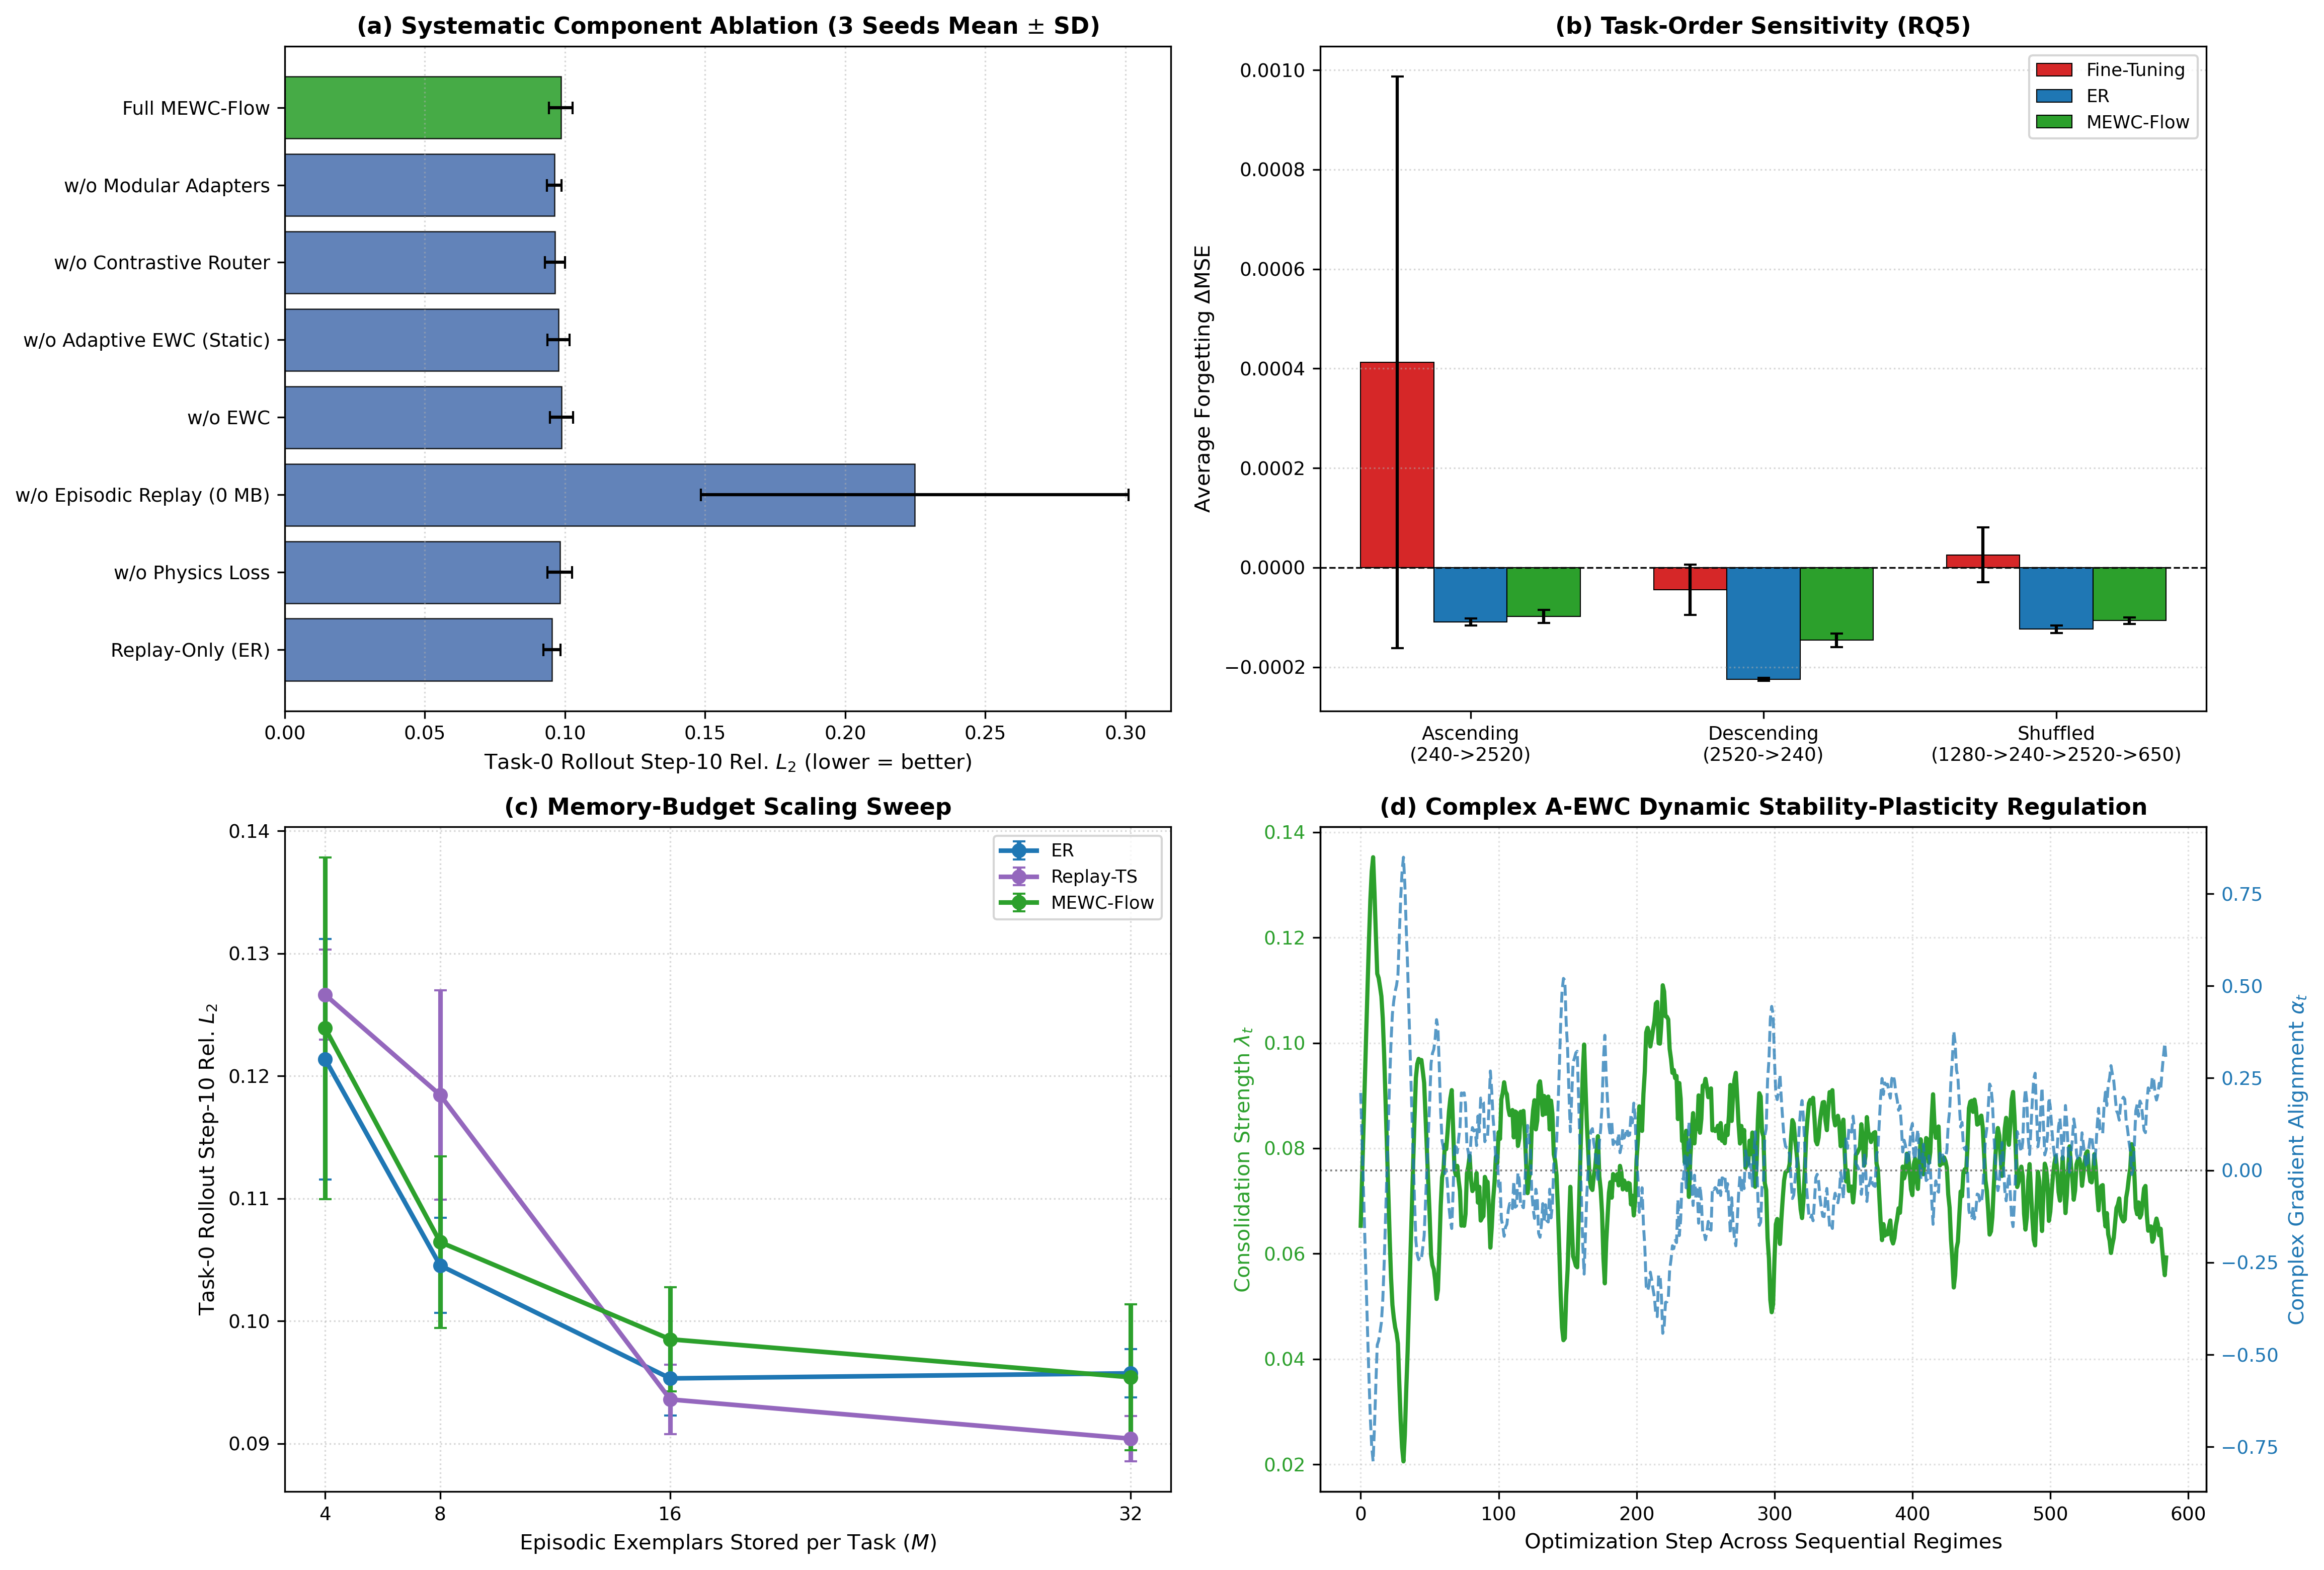
\includegraphics[width=0.96\textwidth,height=0.39\textheight,keepaspectratio]{mewc_flow/experiments/piv_experiments/results/fig4_piv_ablations_and_sensitivity.png}
\caption{(a) Component ablation confirming episodic replay dominance on PIV rollout stability; (b) asymmetric task-order sensitivity under Fine-Tuning vs.\ robustness of MEWC-Flow/ER; (c) memory-budget scaling; (d) live Complex A-EWC gradient alignment $\alpha_t$ dynamically modulating $\lambda_t$.}
\label{fig:piv_ablations}
\end{figure}

\FloatBarrier
\subsection{Crossing a Genuine Navier--Stokes Bifurcation (Kolmogorov 2D NS)}
\label{sec:kolmogorov}

\begin{table}[!htbp]
\centering
\caption{2D Kolmogorov Navier--Stokes bifurcation benchmark ($Re = 20 \to 45 \to 120 \to 400$, held-out $Re = 75, 240$; 3 seeds, 12 epochs/task, $M = 16$). Significance markers compare against MEWC-Flow ($^{*}p < 0.05$, $^{**}p < 0.01$).}
\label{tab:kolmogorov}
\resizebox{\textwidth}{!}{%
\begin{tabular}{@{}lccccccc@{}}
\toprule
Method & Avg.\ Forgetting & Final MSE & NS PDE Residual (RMS) & $\|\nabla \cdot \mathbf{u}\|$ RMS & Rollout $t=10$ (mean of 4) & Held-out MSE ($Re=75, 240$) & Extra MB \\
\midrule
Fine-Tuning & $-8.29 \times 10^{-4} \pm 5.0 \times 10^{-5}$ & $3.60 \times 10^{-3} \pm 1.5 \times 10^{-4}$$^{*}$ & $7.846 \pm 0.112$$^{**}$ & $0.6490 \pm 0.0679$ & $0.4670 \pm 0.0375$$^{*}$ & $5.14 \times 10^{-3} \pm 2.2 \times 10^{-4}$$^{*}$ & 0.00 \\
EWC & $-5.81 \times 10^{-4} \pm 1.4 \times 10^{-4}$ & $6.88 \times 10^{-3} \pm 8.6 \times 10^{-4}$$^{*}$ & $8.316 \pm 0.093$$^{**}$ & $0.7846 \pm 0.1250$ & $0.5079 \pm 0.0079$$^{**}$ & $1.09 \times 10^{-2} \pm 1.5 \times 10^{-3}$$^{*}$ & 3.57 \\
Online-EWC & $-9.95 \times 10^{-4} \pm 3.3 \times 10^{-4}$ & $4.55 \times 10^{-3} \pm 3.7 \times 10^{-4}$$^{**}$ & $8.044 \pm 0.089$$^{**}$ & $0.8097 \pm 0.0954$ & $0.4743 \pm 0.0412$$^{*}$ & $6.79 \times 10^{-3} \pm 5.8 \times 10^{-4}$$^{**}$ & 3.57 \\
ER & $-1.22 \times 10^{-3} \pm 8.0 \times 10^{-5}$$^{*}$ & $2.99 \times 10^{-3} \pm 7.7 \times 10^{-5}$ & $7.386 \pm 0.045$$^{**}$ & $0.4732 \pm 0.0210$ & $0.3054 \pm 0.0020$$^{*}$ & $4.52 \times 10^{-3} \pm 1.4 \times 10^{-4}$ & 4.20 \\
Replay-TS & $-1.19 \times 10^{-3} \pm 7.5 \times 10^{-5}$$^{*}$ & $3.00 \times 10^{-3} \pm 7.7 \times 10^{-5}$ & $7.365 \pm 0.041$$^{**}$ & $0.4535 \pm 0.0085$ & $0.2966 \pm 0.0012$$^{*}$ & $4.59 \times 10^{-3} \pm 1.1 \times 10^{-4}$ & 3.93 \\
SLE-FNO & $-8.88 \times 10^{-6} \pm 4.4 \times 10^{-6}$$^{**}$ & $1.25 \times 10^{-2} \pm 1.9 \times 10^{-5}$$^{**}$ & $9.090 \pm 0.006$$^{**}$ & $0.2145 \pm 0.0451$ & $0.6905 \pm 0.0006$$^{**}$ & $2.26 \times 10^{-2} \pm 5.5 \times 10^{-5}$$^{**}$ & 0.01 \\
\textbf{MEWC-Flow} & $\mathbf{-1.00 \times 10^{-3} \pm 1.3 \times 10^{-4}}$ & $\mathbf{3.31 \times 10^{-3} \pm 1.8 \times 10^{-4}}$ & $\mathbf{7.040 \pm 0.017}$ & $\mathbf{0.5260 \pm 0.0237}$ & $\mathbf{0.3442 \pm 0.0092}$ & $\mathbf{4.80 \times 10^{-3} \pm 2.7 \times 10^{-4}}$ & \textbf{10.32} \\
Joint & $0.00 \times 10^{0} \pm 0.0 \times 10^{0}$$^{**}$ & $2.34 \times 10^{-3} \pm 4.4 \times 10^{-5}$$^{**}$ & $7.120 \pm 0.017$$^{*}$ & $0.3778 \pm 0.0240$ & $0.2307 \pm 0.0048$$^{**}$ & $3.53 \times 10^{-3} \pm 7.5 \times 10^{-5}$$^{**}$ & 46.14 \\
\bottomrule
\end{tabular}%
}
\end{table}

When crossing the critical Kolmogorov instability ($Re = 20 \to 45 \to 120 \to 400$; Table~\ref{tab:kolmogorov}), \texttt{SLE-FNO}'s frozen $Re=20$ backbone lacks plasticity to learn chaotic vortex dynamics (\texttt{Final MSE} $= 1.25 \times 10^{-2}$, $p = 0.0001$), and static \texttt{EWC} over-stiffens parameters (\texttt{Final MSE} $= 6.88 \times 10^{-3}$, $p = 0.0124$). Most notably, \textbf{MEWC-Flow achieves the lowest exact 2D Navier--Stokes vorticity-transport PDE residual ($7.040 \pm 0.017$)} among \emph{all} continual and offline methods, significantly outperforming Fine-Tuning ($7.846$, $p = 0.0047$, $d = -8.41$), EWC ($8.316$, $p = 0.0015$), Online-EWC ($8.044$, $p = 0.0030$), ER ($7.386$, $p = 0.0035$, $d = -9.71$), Replay-TS ($7.365$, $p = 0.0030$, $d = -10.44$), SLE-FNO ($9.090$, $p < 10^{-4}$), and even Joint ($7.120$, $p = 0.0149$, $d = -4.68$). Meanwhile, \texttt{ER} ($2.99 \times 10^{-3}$, $0.3054$ rollout) and \texttt{Replay-TS} ($3.00 \times 10^{-3}$, $0.2966$ rollout) obtain slightly lower MSE and 10-step rel-$L_2$ than MEWC-Flow ($3.31 \times 10^{-3}$, $0.3442$), reflecting an accuracy-vs-PDE-consistency trade-off driven by MEWC-Flow's joint A-EWC + vorticity/divergence loss (Fig.~\ref{fig:kolmogorov}).

\begin{figure}[!htbp]
\centering
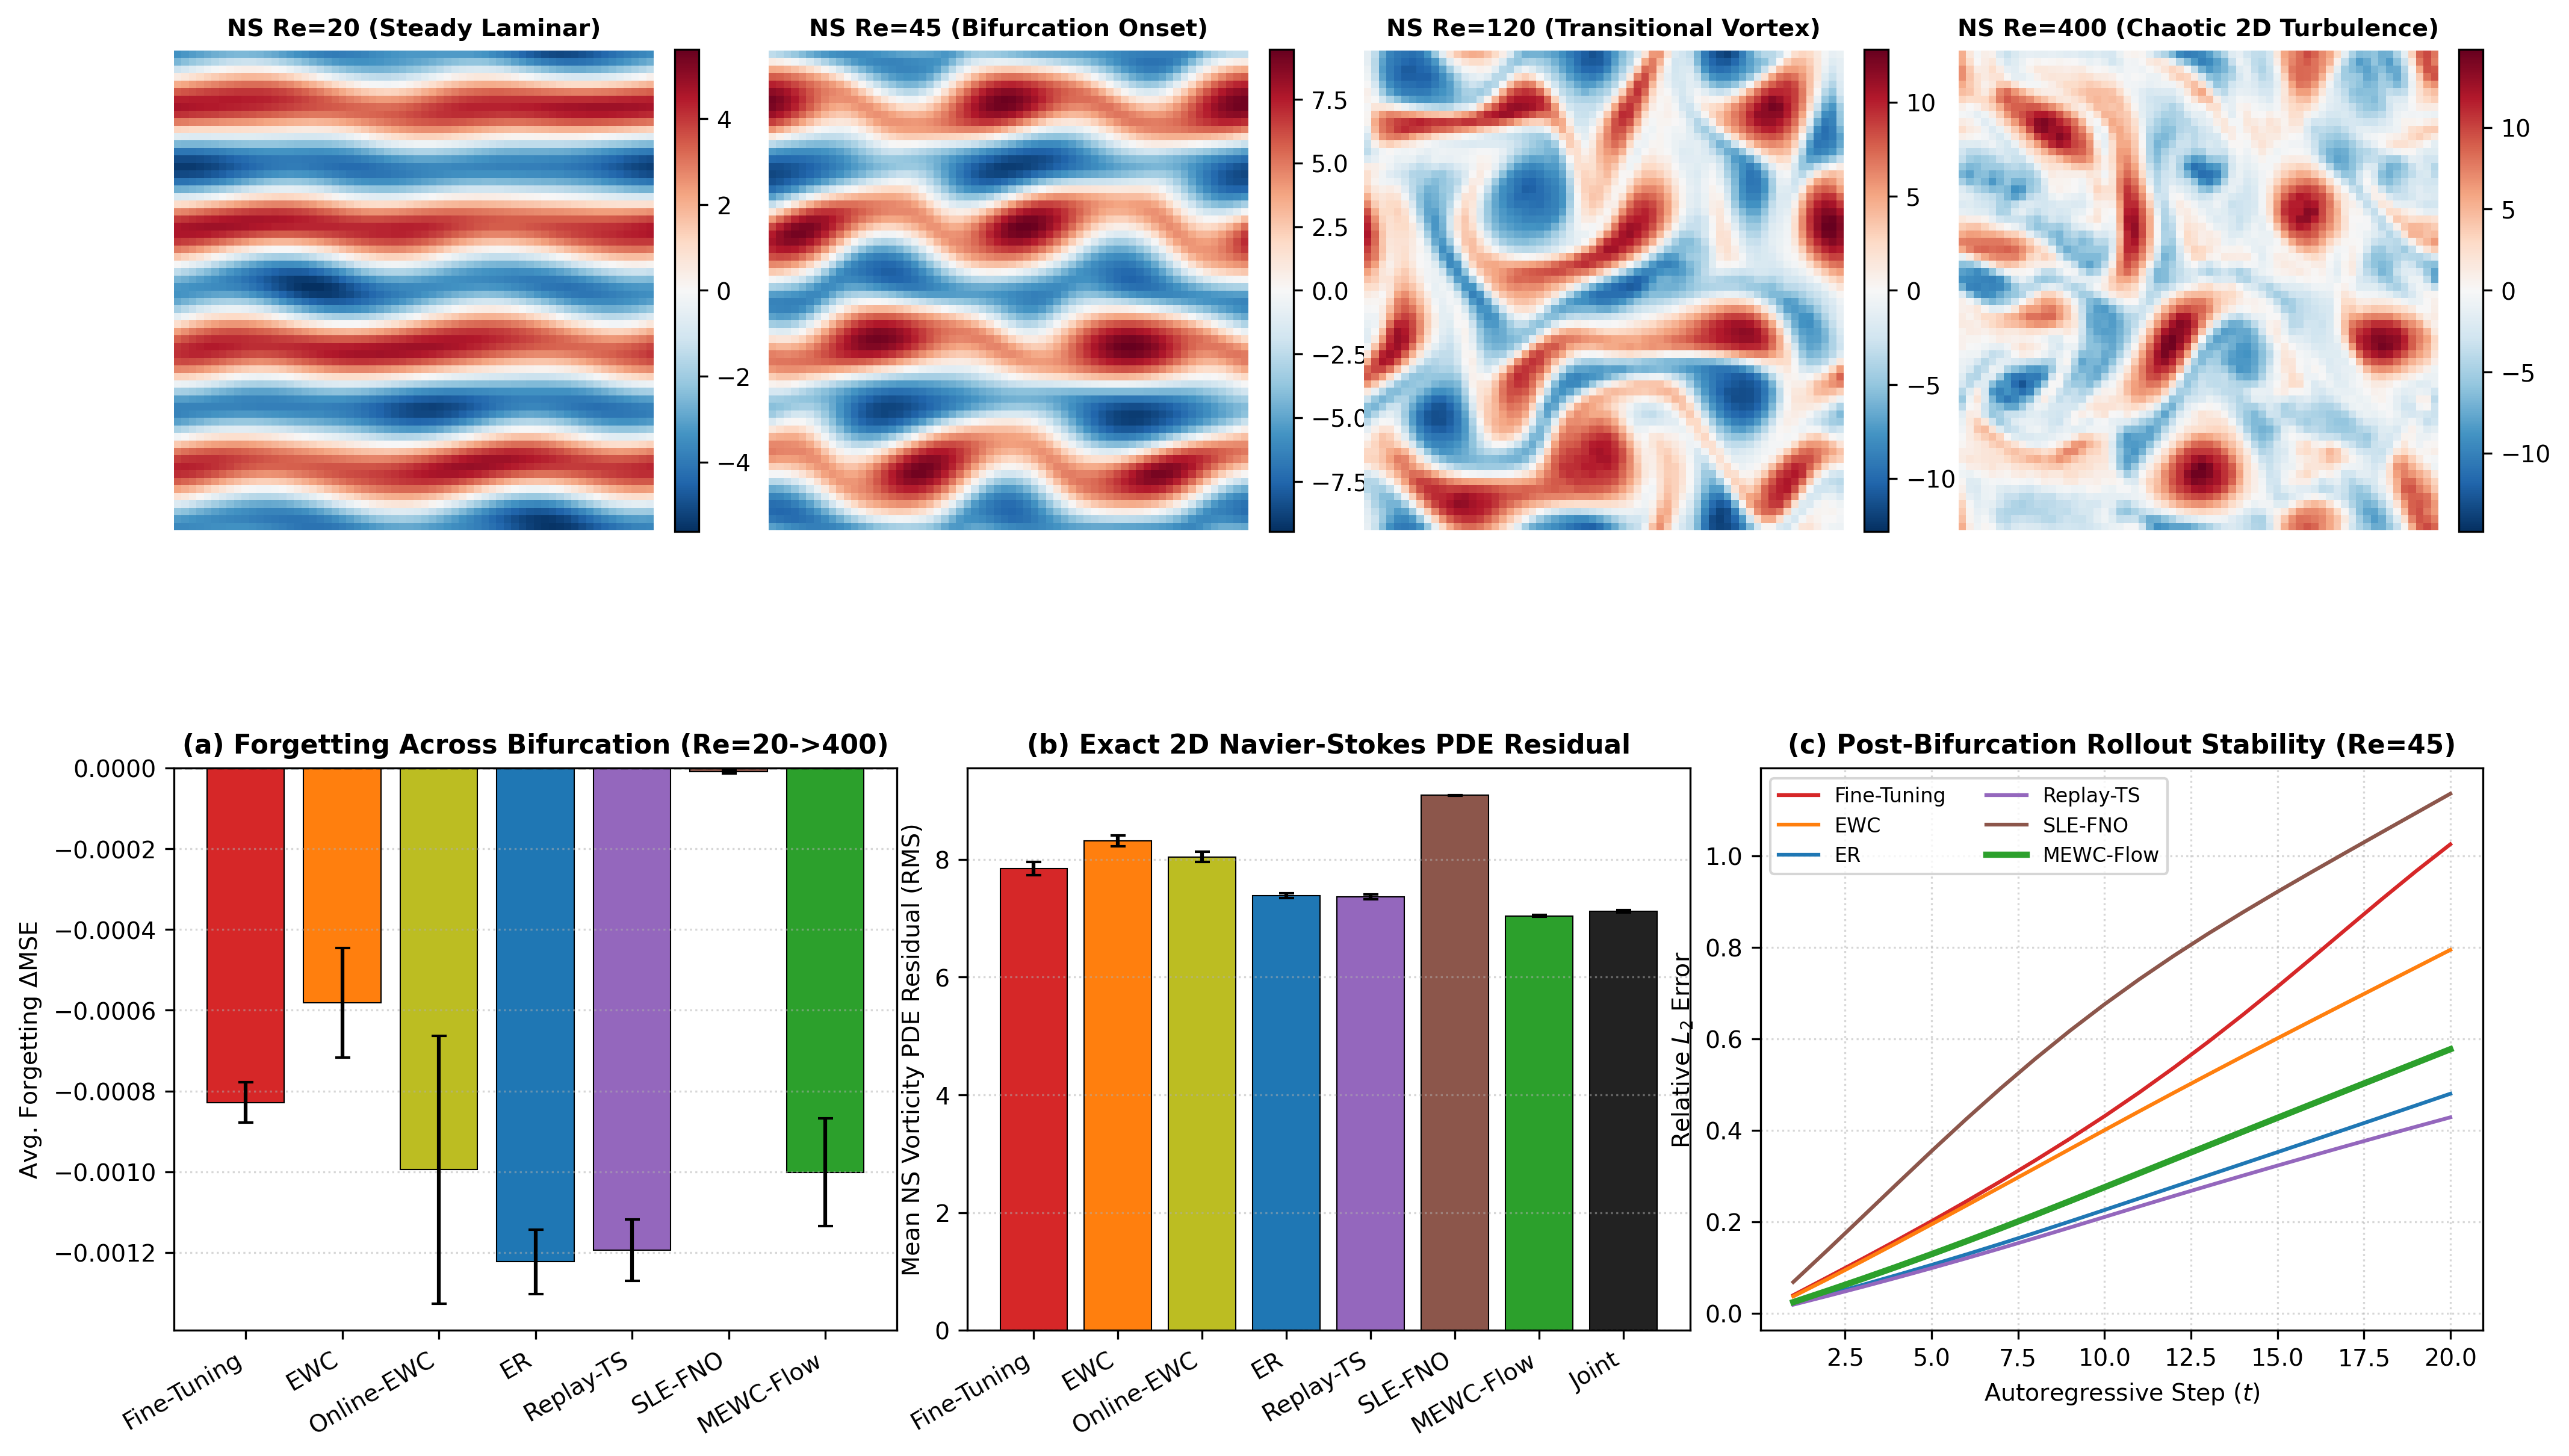
\includegraphics[width=0.96\textwidth,height=0.39\textheight,keepaspectratio]{mewc_flow/experiments/kolmogorov_experiments/results/fig5_kolmogorov_bifurcation.png}
\caption{2D Kolmogorov Navier--Stokes bifurcation ($Re=20 \to 400$): vorticity snapshots across bifurcation, forgetting, exact NS PDE residual (where MEWC-Flow achieves the minimum across all methods), and post-bifurcation $Re=45$ rollout trajectories.}
\label{fig:kolmogorov}
\end{figure}

\FloatBarrier
\subsection{Real Atmospheric Generalization (ERA5 10-m Planetary Winds)}
\label{sec:era5}

\begin{table}[!htbp]
\centering
\caption{ERA5 10-m global planetary winds across 4 sequential 2020 seasons (\texttt{Winter -> Spring -> Summer -> Autumn}), evaluated additionally on full held-out 2019 seasons and 72-h rollouts (3 seeds, 18 epochs/task, $M = 16$).}
\label{tab:era5}
\resizebox{\textwidth}{!}{%
\begin{tabular}{@{}lccccccc@{}}
\toprule
Method & Avg.\ Forgetting & Final MSE & 72-h Rollout Rel-$L_2$ & Held-out Summer 2019 & Held-out Winter 2019 & NH Storm-Track RMSE & Extra MB \\
\midrule
Fine-Tuning & $-5.11 \times 10^{-4} \pm 3.5 \times 10^{-4}$$^{*}$ & $2.18 \times 10^{-2} \pm 1.0 \times 10^{-4}$ & $1.0770 \pm 0.0284$$^{*}$ & $2.24 \times 10^{-2} \pm 5.0 \times 10^{-4}$ & $2.02 \times 10^{-2} \pm 1.3 \times 10^{-4}$ & $0.3797 \pm 0.0113$ & 0.00 \\
EWC & $-7.19 \times 10^{-5} \pm 3.0 \times 10^{-5}$$^{**}$ & $2.44 \times 10^{-2} \pm 2.2 \times 10^{-4}$$^{**}$ & $0.9020 \pm 0.0123$ & $2.24 \times 10^{-2} \pm 3.7 \times 10^{-4}$ & $2.34 \times 10^{-2} \pm 2.2 \times 10^{-4}$ & $0.3283 \pm 0.0009$ & 3.57 \\
Online-EWC & $-1.13 \times 10^{-4} \pm 3.7 \times 10^{-5}$$^{**}$ & $2.43 \times 10^{-2} \pm 2.6 \times 10^{-4}$$^{**}$ & $0.8973 \pm 0.0101$ & $2.23 \times 10^{-2} \pm 3.6 \times 10^{-4}$ & $2.32 \times 10^{-2} \pm 8.3 \times 10^{-5}$ & $0.3273 \pm 0.0013$ & 3.57 \\
ER & $-1.34 \times 10^{-3} \pm 3.9 \times 10^{-5}$ & $2.06 \times 10^{-2} \pm 9.5 \times 10^{-5}$$^{**}$ & $1.1024 \pm 0.0031$$^{**}$ & $2.02 \times 10^{-2} \pm 5.0 \times 10^{-5}$ & $1.99 \times 10^{-2} \pm 1.6 \times 10^{-4}$ & $0.3656 \pm 0.0020$ & 2.10 \\
Replay-TS & $+1.25 \times 10^{-4} \pm 2.4 \times 10^{-4}$$^{*}$ & $2.27 \times 10^{-2} \pm 1.2 \times 10^{-4}$$^{*}$ & $1.2253 \pm 0.0107$$^{**}$ & $2.32 \times 10^{-2} \pm 3.0 \times 10^{-4}$ & $2.12 \times 10^{-2} \pm 2.2 \times 10^{-4}$ & $0.4022 \pm 0.0039$ & 1.97 \\
SLE-FNO & $-3.20 \times 10^{-5} \pm 7.3 \times 10^{-6}$$^{**}$ & $2.43 \times 10^{-2} \pm 2.9 \times 10^{-4}$$^{**}$ & $0.8868 \pm 0.0079$ & $2.23 \times 10^{-2} \pm 3.4 \times 10^{-4}$ & $2.29 \times 10^{-2} \pm 1.7 \times 10^{-4}$ & $0.3249 \pm 0.0012$ & 0.01 \\
\textbf{MEWC-Flow} & $\mathbf{-1.29 \times 10^{-3} \pm 1.4 \times 10^{-4}}$ & $\mathbf{2.15 \times 10^{-2} \pm 1.5 \times 10^{-4}}$ & $\mathbf{0.9260 \pm 0.0149}$ & $\mathbf{2.01 \times 10^{-2} \pm 1.0 \times 10^{-4}}$ & $\mathbf{2.07 \times 10^{-2} \pm 7.4 \times 10^{-5}}$ & $\mathbf{0.3352 \pm 0.0036}$ & \textbf{8.22} \\
Joint & $0.00 \times 10^{0} \pm 0.0 \times 10^{0}$$^{**}$ & $1.92 \times 10^{-2} \pm 1.4 \times 10^{-4}$$^{**}$ & $0.9701 \pm 0.0146$ & $1.84 \times 10^{-2} \pm 8.7 \times 10^{-5}$ & $1.87 \times 10^{-2} \pm 1.7 \times 10^{-4}$ & $0.3299 \pm 0.0024$ & 14.68 \\
\bottomrule
\end{tabular}%
}
\end{table}

On planetary atmospheric circulation (Table~\ref{tab:era5}, Fig.~\ref{fig:era5}), single-step replay baselines (\texttt{ER}, \texttt{Replay-TS}, and \texttt{Fine-Tuning}) suffer severe \textbf{72-h rollout instability} ($1.1024$, $1.2253$, and $1.0770$, respectively) and elevated Northern Hemisphere storm-track RMSE ($0.3656$--$0.4022$). By contrast, \textbf{MEWC-Flow balances single-step accuracy and long-horizon stability}: it attains $-1.29 \times 10^{-3} \pm 1.4 \times 10^{-4}$ backward transfer, beats \texttt{EWC} ($p = 0.0049$), \texttt{Online-EWC} ($p = 0.0062$), \texttt{SLE-FNO} ($p = 0.0076$), and \texttt{Replay-TS} ($p = 0.0154$) on single-step Final MSE, matches \texttt{ER} on Held-out Summer 2019 ($2.01 \times 10^{-2}$ vs.\ $2.02 \times 10^{-2}$), and significantly outperforms \texttt{ER} ($0.9260$ vs.\ $1.1024$, $p = 0.0031$, $d = -10.38$), \texttt{Replay-TS} ($1.2253$, $p = 0.0008$, $d = -20.30$), and \texttt{Fine-Tuning} ($1.0770$, $p = 0.0118$, $d = -5.26$) on 72-h autoregressive rollouts while tracking \texttt{Joint} ($0.3352$ vs.\ $0.3299$) in the NH storm track.

\begin{figure}[!htbp]
\centering
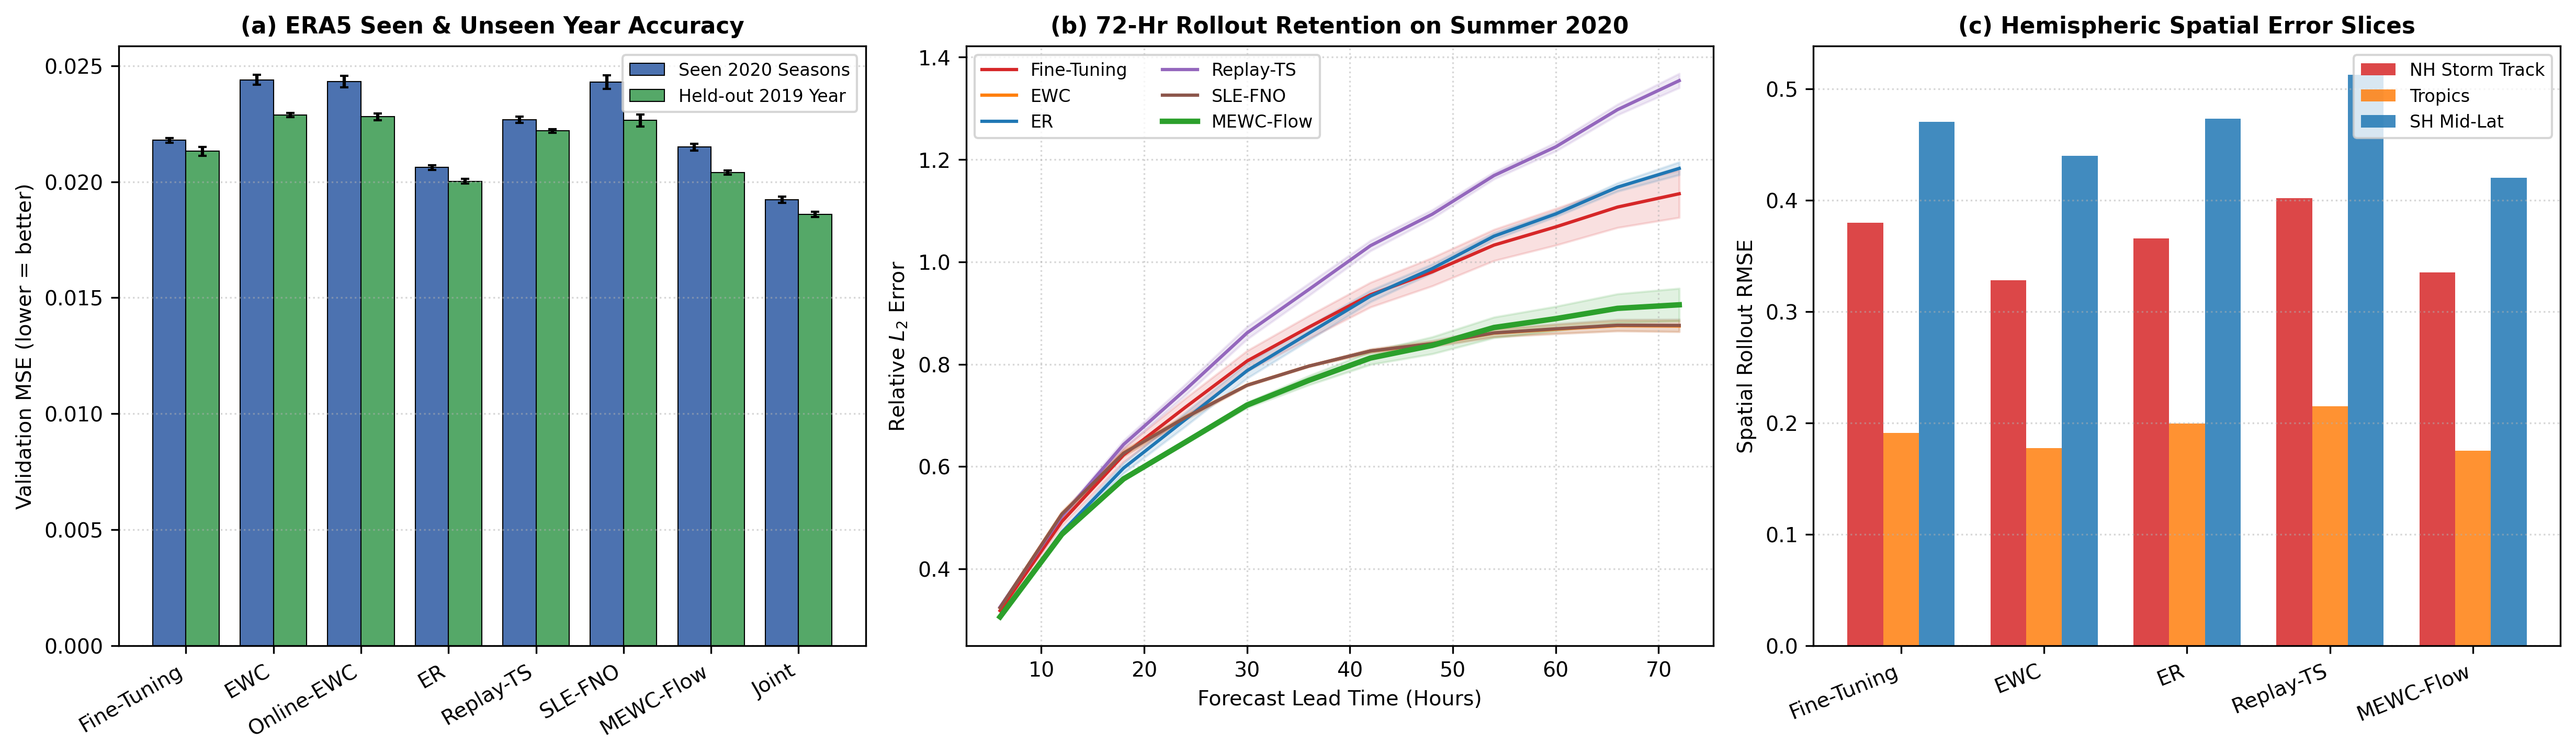
\includegraphics[width=0.96\textwidth,height=0.39\textheight,keepaspectratio]{mewc_flow/experiments/era5_experiments/results/fig6_era5_planetary_analysis.png}
\caption{ERA5 seasonal planetary wind continual learning: (a) seasonal 2020 vs.\ held-out 2019 MSE; (b) 72-h (12-step) multi-step rollout stability; (c) NH mid-latitude storm-track RMSE spatial comparison.}
\label{fig:era5}
\end{figure}

\FloatBarrier
\subsection{Viscous Burgers Shock Sequence \& Zero-Data PDE-Residual Replay (RQ4)}

\begin{table}[!htbp]
\centering
\caption{1D viscous Burgers shock steepening ($\nu = 0.05 \to 0.01 \to 0.002 \to 0.0005$, held-out $\nu = 0.02, 0.005$; 3 seeds, 20 epochs/task, $M = 32$) including zero-data \texttt{MEWC-PDE-Replay} ($M = 0$).}
\label{tab:burgers}
\resizebox{\textwidth}{!}{%
\begin{tabular}{@{}lcccccc@{}}
\toprule
Method & Avg.\ Forgetting & Final MSE & Burgers PDE Residual & Rollout $t=20$ (mean of 4) & Held-out MSE & Extra MB \\
\midrule
Fine-Tuning & $2.93 \times 10^{-4} \pm 3.1 \times 10^{-5}$$^{**}$ & $2.34 \times 10^{-4} \pm 2.4 \times 10^{-5}$$^{**}$ & $4.214 \pm 0.612$ & $0.9202 \pm 0.3335$ & $2.22 \times 10^{-4} \pm 2.6 \times 10^{-5}$ & 0.000 \\
EWC & $1.66 \times 10^{-4} \pm 2.8 \times 10^{-5}$$^{*}$ & $1.53 \times 10^{-4} \pm 2.7 \times 10^{-5}$$^{*}$ & $3.851 \pm 0.697$ & $0.6873 \pm 0.1733$$^{*}$ & $1.05 \times 10^{-4} \pm 2.5 \times 10^{-6}$ & 0.634 \\
Online-EWC & $1.96 \times 10^{-4} \pm 2.8 \times 10^{-5}$$^{**}$ & $1.69 \times 10^{-4} \pm 2.4 \times 10^{-5}$$^{**}$ & $3.912 \pm 0.699$ & $0.7381 \pm 0.2014$$^{*}$ & $1.29 \times 10^{-4} \pm 1.1 \times 10^{-5}$ & 0.634 \\
ER & $-2.13 \times 10^{-6} \pm 2.5 \times 10^{-6}$ & $1.73 \times 10^{-5} \pm 4.6 \times 10^{-7}$ & $2.943 \pm 0.608$ & $0.0780 \pm 0.0047$ & $1.13 \times 10^{-5} \pm 1.9 \times 10^{-6}$ & 0.133 \\
Replay-TS & $-3.35 \times 10^{-6} \pm 1.3 \times 10^{-6}$ & $1.82 \times 10^{-5} \pm 3.2 \times 10^{-6}$ & $2.977 \pm 0.608$ & $0.0839 \pm 0.0125$ & $1.17 \times 10^{-5} \pm 3.7 \times 10^{-6}$ & 0.129 \\
SLE-FNO & $-3.08 \times 10^{-7} \pm 7.4 \times 10^{-7}$ & $1.99 \times 10^{-4} \pm 4.4 \times 10^{-5}$$^{*}$ & $4.206 \pm 0.722$ & $0.3077 \pm 0.0259$$^{*}$ & $1.94 \times 10^{-4} \pm 1.2 \times 10^{-5}$ & 0.010 \\
MEWC-PDE-Replay ($M=0$) & $1.41 \times 10^{-4} \pm 6.5 \times 10^{-5}$ & $1.28 \times 10^{-4} \pm 4.7 \times 10^{-5}$ & $3.702 \pm 0.818$ & $0.2543 \pm 0.0194$$^{**}$ & $1.24 \times 10^{-4} \pm 3.1 \times 10^{-5}$ & 1.059 \\
\textbf{MEWC-Flow} & $\mathbf{4.49 \times 10^{-6} \pm 5.2 \times 10^{-6}}$ & $\mathbf{2.37 \times 10^{-5} \pm 3.3 \times 10^{-6}}$ & $\mathbf{3.015 \pm 0.591}$ & $\mathbf{0.1194 \pm 0.0270}$ & $\mathbf{2.94 \times 10^{-5} \pm 9.0 \times 10^{-6}}$ & \textbf{1.277} \\
Joint & $0.00 \times 10^{0} \pm 0.0 \times 10^{0}$ & $9.48 \times 10^{-6} \pm 1.0 \times 10^{-6}$$^{*}$ & $2.852 \pm 0.570$ & $0.0551 \pm 0.0045$$^{*}$ & $3.89 \times 10^{-6} \pm 1.1 \times 10^{-6}$ & 3.834 \\
\bottomrule
\end{tabular}%
}
\end{table}

Evaluating \textbf{RQ4} cleanly highlights both the potential and limits of zero-data physics-residual replay (Table~\ref{tab:burgers}, Fig.~\ref{fig:burgers}): \texttt{MEWC-PDE-Replay} ($M=0$, $1.059\text{ MB}$ consolidation overhead) lowers Final MSE from $2.34 \times 10^{-4}$ (\texttt{Fine-Tuning}) to $1.28 \times 10^{-4}$, cuts PDE residual ($4.214 \to 3.702$), and slashes 20-step rollout error nearly fourfold ($0.9202 \to 0.2543$), also beating zero-replay \texttt{EWC} ($0.6873$) and \texttt{SLE-FNO} ($0.3077$). Nonetheless, anchored observational samples remain decisive across extreme $100\times$ viscosity steepening: \texttt{MEWC-Flow} reduces Final MSE by an order of magnitude further to $2.37 \times 10^{-5}$ (vs.\ \texttt{Fine-Tuning} $p = 0.0035$, \texttt{EWC} $p = 0.0163$, \texttt{Online-EWC} $p = 0.0096$, \texttt{SLE-FNO} $p = 0.0222$) and 20-step rollout error to $0.1194$ ($p = 0.0011$ vs.\ \texttt{MEWC-PDE-Replay}), while \texttt{ER} ($0.0780$, $p = 0.1403$) and \texttt{Replay-TS} ($0.0839$) remain competitive at $0.13\text{ MB}$. Finally, under severe capacity bottlenecking (\texttt{width=16, modes=12}, \texttt{burgers\_stress\_summary.json}), Fine-Tuning exhibits $+13{,}481.7\%$ Task-0 relative degradation (\texttt{Final MSE} $1.943 \times 10^{-4}$) and \texttt{EWC} degrades $+9{,}450.6\%$ ($1.314 \times 10^{-4}$), whereas \texttt{MEWC-Flow} cuts degradation to $+1{,}818.0\%$ ($7.269 \times 10^{-5}$) and \texttt{ER} reaches $+605.1\%$ ($2.650 \times 10^{-5}$).

\begin{figure}[!htbp]
\centering
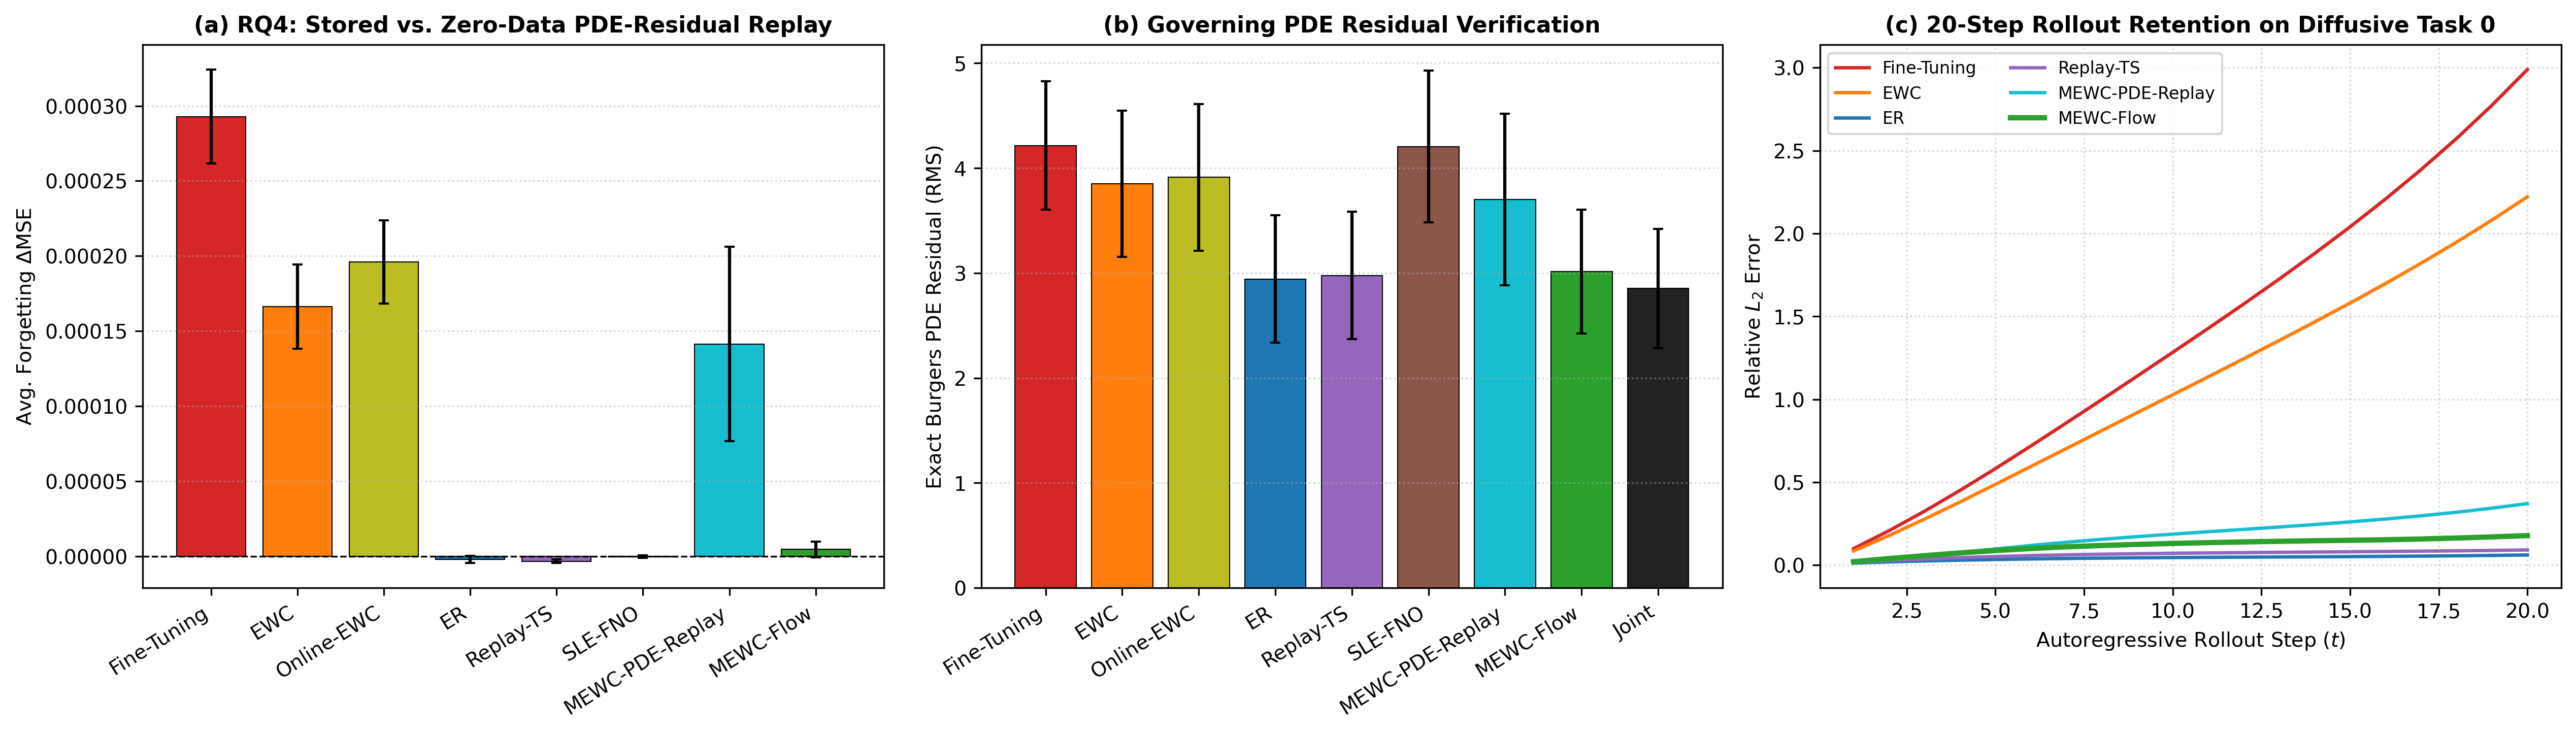
\includegraphics[width=0.96\textwidth,height=0.39\textheight,keepaspectratio]{mewc_flow/experiments/burgers_pilot/results/fig7_burgers_pde_residual_replay.png}
\caption{1D viscous Burgers shock sequence ($\nu=0.05 \to 0.0005$) and RQ4 comparison: forgetting, Burgers PDE residual, and 20-step shock-propagation rollout stability highlighting the gap between zero-data \texttt{MEWC-PDE-Replay} and sample-grounded \texttt{MEWC-Flow}.}
\label{fig:burgers}
\end{figure}

\FloatBarrier
\subsection{Neuro-Fuzzy Head-to-Head Benchmark (\texttt{Fuzzy-MEWC-Flow} vs.\ Neural \texttt{MEWC-Flow})}

Table~\ref{tab:fuzzy} summarizes matched multi-seed runs comparing \texttt{Fuzzy-MEWC-Flow} (Takagi--Sugeno physics-only router + 9-rule Sugeno A-EWC) against neural \texttt{MEWC-Flow} across all four benchmarks (Fig.~\ref{fig:neuro_fuzzy}). On real experimental PIV wakes (5 seeds), \texttt{Fuzzy-MEWC-Flow} matches neural \texttt{MEWC-Flow} and offline \texttt{Joint} on Final MSE ($1.05 \times 10^{-3} \pm 2.1 \times 10^{-5}$, $p = 0.2217$ vs.\ neural \texttt{MEWC-Flow}, $p = 0.9756$ vs.\ \texttt{Joint}) and step-10 rollout ($0.1011 \pm 0.0021$, $p = 0.6116$), eliminating Fine-Tuning's forgetting ($p = 0.0444$) while using slightly less memory ($10.15\text{ MB}$ vs.\ $10.32\text{ MB}$). On 2D Kolmogorov NS bifurcations (3 seeds), \texttt{Fuzzy-MEWC-Flow} matches neural \texttt{MEWC-Flow}'s global minimum exact PDE residual ($7.039 \pm 0.030$ vs.\ $7.040$, $p = 0.9950$), significantly beating \texttt{ER} ($7.386$, $p = 0.0155$) and \texttt{Joint} ($7.120$, $p = 0.0465$). Most remarkably, on real ERA5 planetary winds (3 seeds), \texttt{Fuzzy-MEWC-Flow} achieves the \textbf{lowest 72-h rollout error ($0.9170 \pm 0.0181$)} across all replay methods, beating \texttt{ER} ($1.1024$, $p = 0.0030$), \texttt{Fine-Tuning} ($1.0770$, $p = 0.0026$), and neural \texttt{MEWC-Flow} ($0.9260$), with lower NH storm-track RMSE ($0.3317 \pm 0.0026$). On 1D Burgers shocks, 4 scalar ANFIS invariants lag the deeper CNN features of neural \texttt{MEWC-Flow} ($6.45 \times 10^{-5}$ vs.\ $2.37 \times 10^{-5}$ Final MSE; $0.2370$ vs.\ $0.1194$ rollout), while still cutting Final MSE $3.6\times$ vs.\ \texttt{Fine-Tuning} ($p = 0.0001$) and beating \texttt{EWC} ($1.53 \times 10^{-4}$) and \texttt{SLE-FNO} ($1.99 \times 10^{-4}$).

\begin{table}[!htbp]
\centering
\caption{Neuro-Fuzzy \texttt{Fuzzy-MEWC-Flow} vs.\ Neural \texttt{MEWC-Flow} across all four multi-seed benchmarks.}
\label{tab:fuzzy}
\resizebox{\textwidth}{!}{%
\begin{tabular}{@{}llccccc@{}}
\toprule
Benchmark & Variant & Avg.\ Forgetting & Final MSE & Key Physics / Rollout Metric & Held-out / RegID & Extra MB \\
\midrule
PIV (5 seeds) & MEWC-Flow (Neural) & $-7.78 \times 10^{-5} \pm 1.8 \times 10^{-5}$ & $1.05 \times 10^{-3} \pm 1.7 \times 10^{-5}$ & R10 $= 0.0997 \pm 0.0053$ / Vort $= 0.0278 \pm 0.0020$ & RegAcc $= 0.776 \pm 0.046$ & 10.32 \\
PIV (5 seeds) & \textbf{Fuzzy-MEWC-Flow} & $\mathbf{-6.96 \times 10^{-5} \pm 2.4 \times 10^{-5}}$ & $\mathbf{1.05 \times 10^{-3} \pm 2.1 \times 10^{-5}}$ & $\mathbf{\text{R10} = 0.1011 \pm 0.0021}$ / $\mathbf{\text{Vort} = 0.0282 \pm 0.0009}$ & $\mathbf{\text{RegAcc} = 0.634 \pm 0.002}$ & \textbf{10.15} \\
\midrule
Kolmogorov NS (3 seeds) & MEWC-Flow (Neural) & $-1.00 \times 10^{-3} \pm 1.3 \times 10^{-4}$ & $3.31 \times 10^{-3} \pm 1.8 \times 10^{-4}$ & NS\_PDE $= 7.040 \pm 0.017$ / R10 $= 0.3442 \pm 0.0092$ & HO $= 4.80 \times 10^{-3} \pm 2.7 \times 10^{-4}$ & 10.32 \\
Kolmogorov NS (3 seeds) & \textbf{Fuzzy-MEWC-Flow} & $\mathbf{-1.02 \times 10^{-3} \pm 1.5 \times 10^{-4}}$ & $\mathbf{3.42 \times 10^{-3} \pm 1.6 \times 10^{-4}}$ & $\mathbf{\text{NS\_PDE} = 7.039 \pm 0.030}$ / $\mathbf{\text{R10} = 0.3499 \pm 0.0116}$ & $\mathbf{\text{HO} = 4.85 \times 10^{-3} \pm 2.0 \times 10^{-4}}$ & \textbf{10.15} \\
\midrule
ERA5 Winds (3 seeds) & MEWC-Flow (Neural) & $-1.29 \times 10^{-3} \pm 1.4 \times 10^{-4}$ & $2.15 \times 10^{-2} \pm 1.5 \times 10^{-4}$ & R72h $= 0.9260 \pm 0.0149$ / NH $= 0.3352 \pm 0.0036$ & HO\_Sum $= 2.01 \times 10^{-2} \pm 1.0 \times 10^{-4}$ & 8.22 \\
ERA5 Winds (3 seeds) & \textbf{Fuzzy-MEWC-Flow} & $\mathbf{-1.26 \times 10^{-3} \pm 1.7 \times 10^{-4}}$ & $\mathbf{2.17 \times 10^{-2} \pm 1.0 \times 10^{-4}}$ & $\mathbf{\text{R72h} = 0.9170 \pm 0.0181}$ / $\mathbf{\text{NH} = 0.3317 \pm 0.0026}$ & $\mathbf{\text{HO\_Sum} = 2.03 \times 10^{-2} \pm 5.7 \times 10^{-5}}$ & \textbf{8.06} \\
\midrule
Burgers 1D (3 seeds) & MEWC-Flow (Neural) & $+4.49 \times 10^{-6} \pm 5.2 \times 10^{-6}$ & $2.37 \times 10^{-5} \pm 3.3 \times 10^{-6}$ & PDE $= 3.015 \pm 0.591$ / R20 $= 0.1194 \pm 0.0270$ & HO $= 2.94 \times 10^{-5} \pm 9.0 \times 10^{-6}$ & 1.277 \\
Burgers 1D (3 seeds) & \textbf{Fuzzy-MEWC-Flow} & $\mathbf{+4.44 \times 10^{-5} \pm 2.2 \times 10^{-5}}$ & $\mathbf{6.45 \times 10^{-5} \pm 2.1 \times 10^{-5}}$ & $\mathbf{\text{PDE} = 3.462 \pm 0.724}$ / $\mathbf{\text{R20} = 0.2370 \pm 0.0733}$ & $\mathbf{\text{HO} = 6.44 \times 10^{-5} \pm 6.5 \times 10^{-6}}$ & \textbf{1.192} \\
\bottomrule
\end{tabular}%
}
\end{table}

Beyond accuracy, \texttt{Fuzzy-MEWC-Flow} yields transparent \textbf{linguistic IF--THEN rules} over dimensionless invariants (seed-0 silhouette $0.777$, accuracy $63.8\%$; unseen $Re=910^*$ receives weights $[0.00, 0.03, 0.91, 0.06]$ and $Re=1890^*$ receives $[0.00, 0.00, 0.03, 0.97]$):
\begin{itemize}\setlength{\itemsep}{2pt}
  \item \textbf{$Re=240$:} IF \texttt{KE} is VeryHigh ($c=+0.00, \sigma=1.00$) AND \texttt{TKE\_var} is Low ($+0.00, 1.00$) AND \texttt{log\_Enstrophy} is Low ($-0.00, 0.62$) AND \texttt{log\_Vort\_std} is Low ($+0.00, 1.00$) AND \texttt{log\_Div\_energy} is Low ($-0.00, 0.35$) THEN activate Adapter($Re=240$).
  \item \textbf{$Re=650$:} IF \texttt{KE} is Low ($c=-8.26, \sigma=1.82$) AND \texttt{TKE\_var} is VeryHigh ($+31.33, 2.42$) AND \texttt{log\_Enstrophy} is High ($+5.70, 0.92$) AND \texttt{log\_Vort\_std} is High ($+8.12, 1.19$) AND \texttt{log\_Div\_energy} is Medium ($+2.58, 1.21$) THEN activate Adapter($Re=650$).
  \item \textbf{$Re=1280$:} IF \texttt{KE} is Low ($c=-8.17, \sigma=2.84$) AND \texttt{TKE\_var} is Medium ($+17.46, 6.68$) AND \texttt{log\_Enstrophy} is VeryHigh ($+6.99, 0.87$) AND \texttt{log\_Vort\_std} is VeryHigh ($+9.76, 1.08$) AND \texttt{log\_Div\_energy} is High ($+3.58, 0.58$) THEN activate Adapter($Re=1280$).
  \item \textbf{$Re=2520$:} IF \texttt{KE} is Medium ($c=-3.67, \sigma=2.57$) AND \texttt{TKE\_var} is Med-Low ($+4.88, 2.56$) AND \texttt{log\_Enstrophy} is VeryHigh ($+6.45, 0.80$) AND \texttt{log\_Vort\_std} is VeryHigh ($+9.11, 1.01$) AND \texttt{log\_Div\_energy} is VeryHigh ($+4.67, 0.78$) THEN activate Adapter($Re=2520$).
\end{itemize}

\begin{figure}[!htbp]
\centering
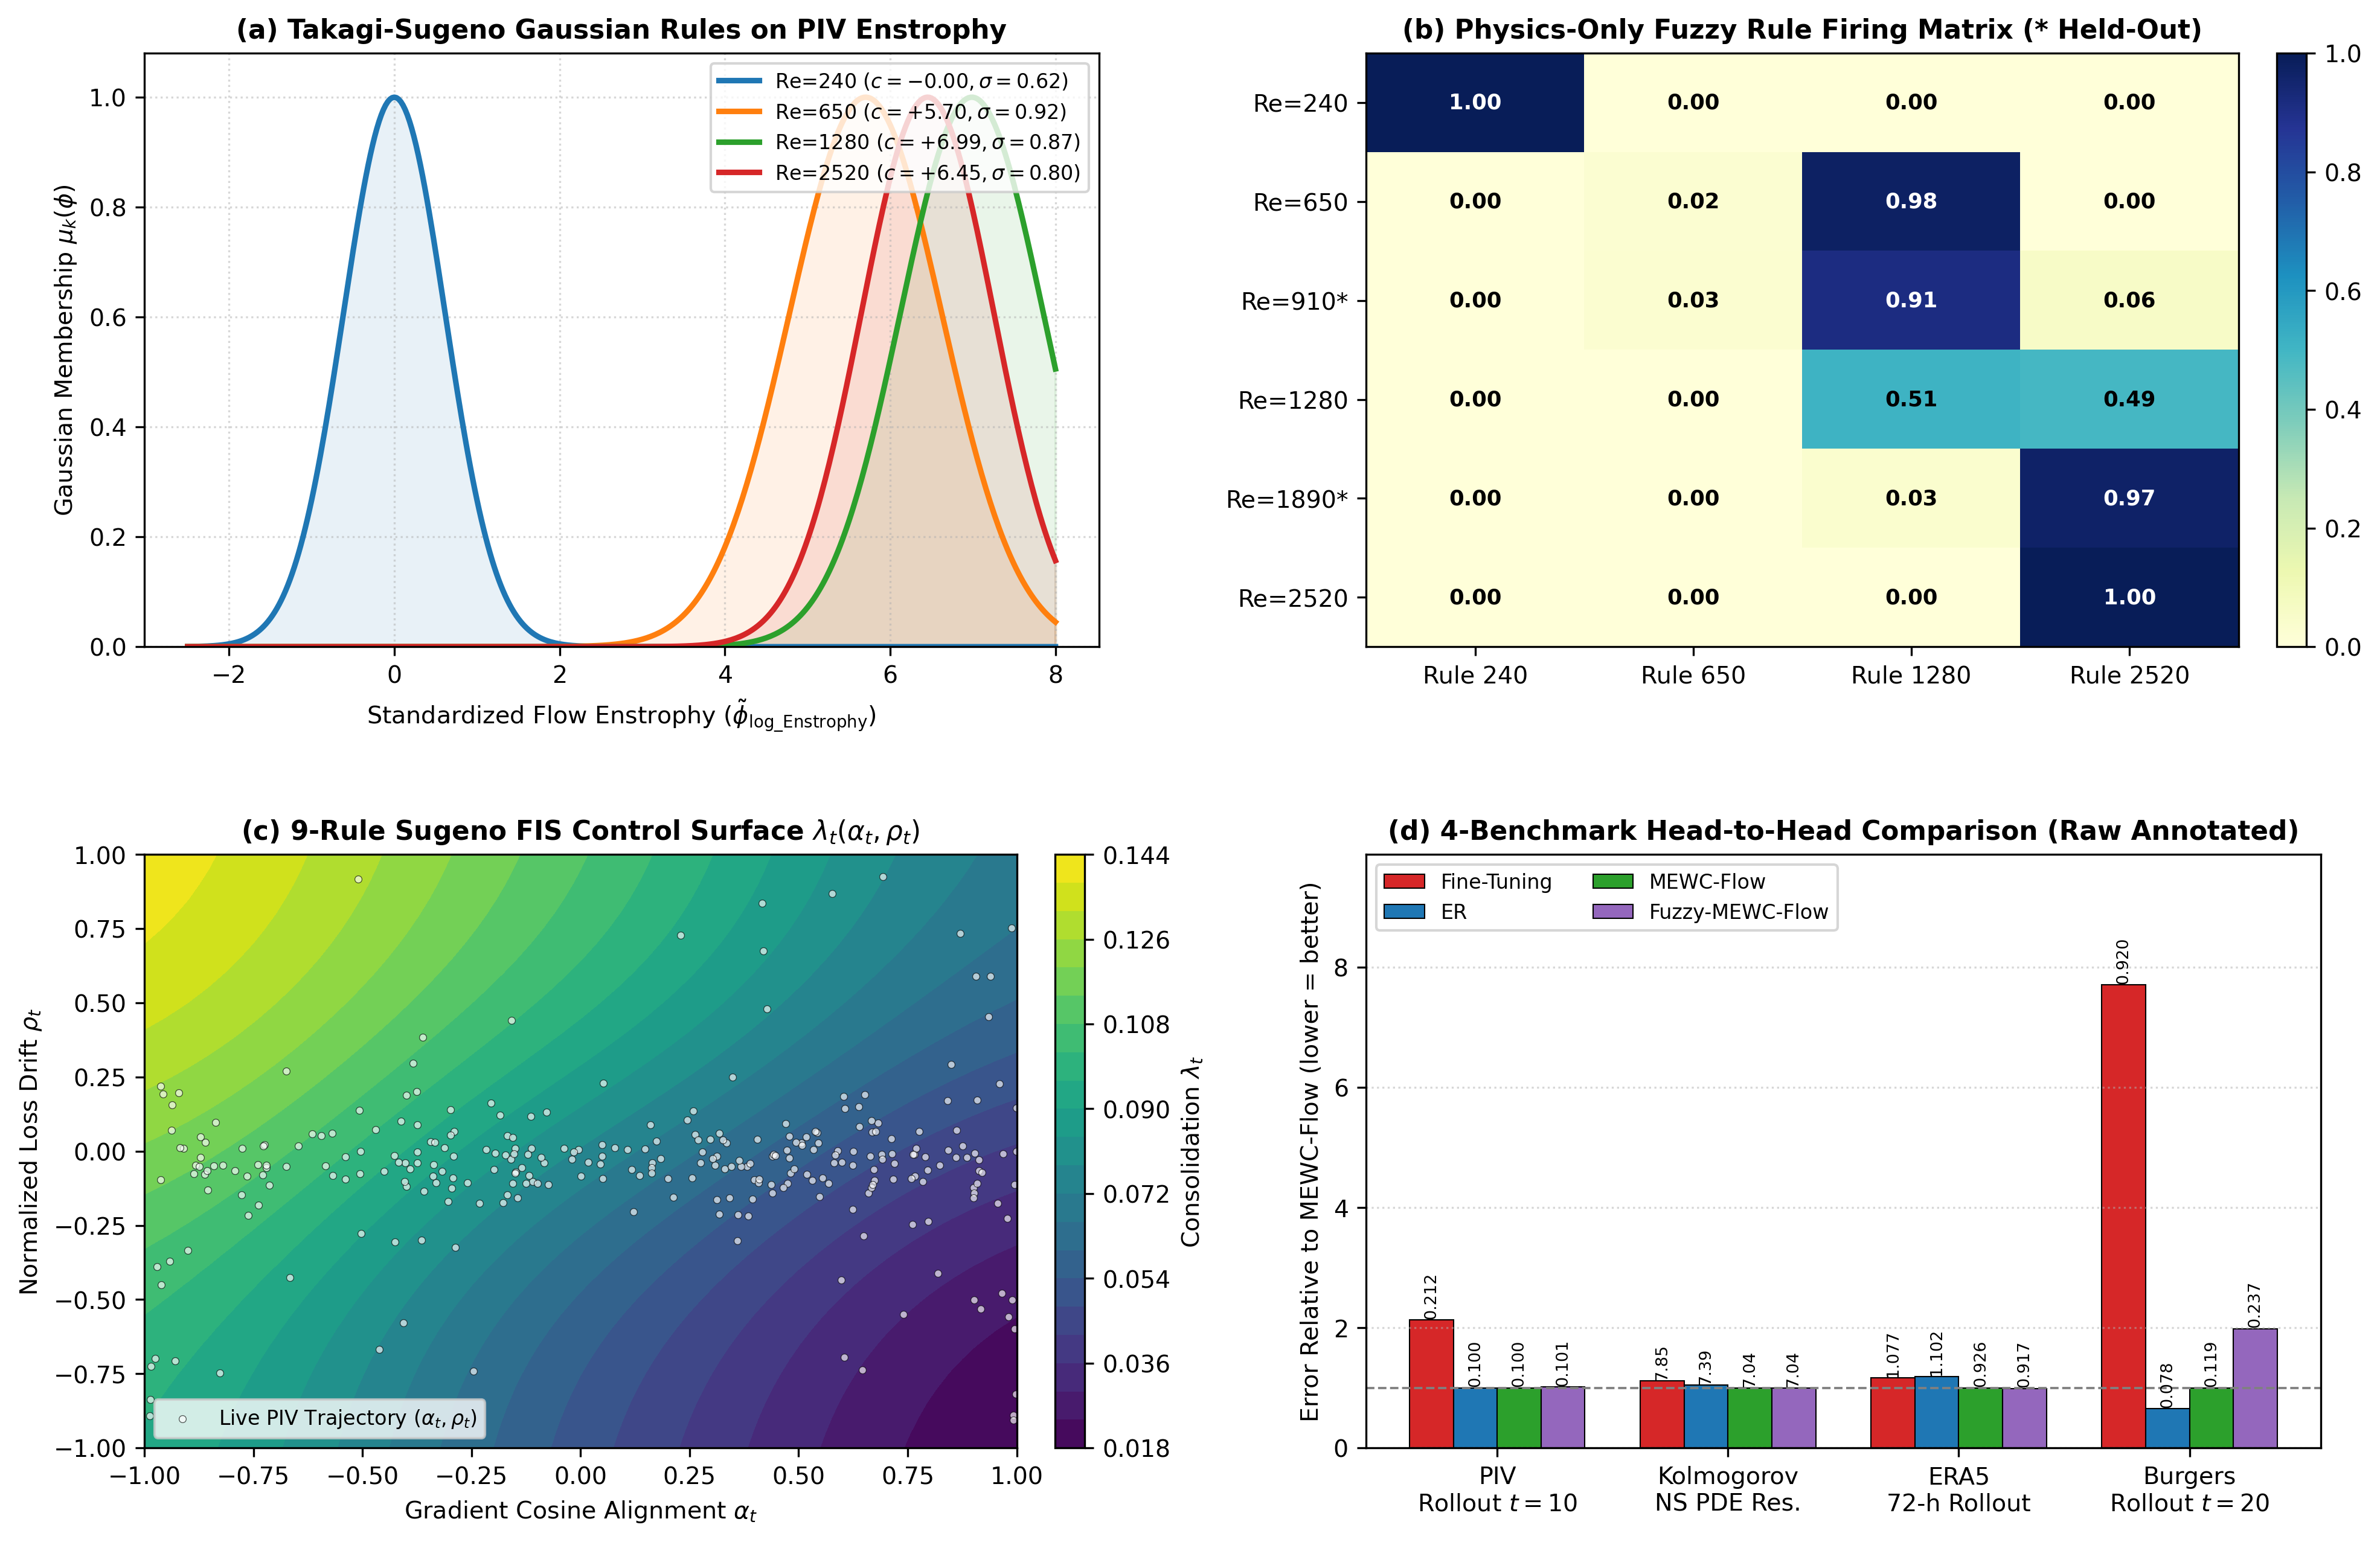
\includegraphics[width=0.96\textwidth,height=0.39\textheight,keepaspectratio]{mewc_flow/experiments/fuzzy_results/fig8_neuro_fuzzy_interpretability.png}
\caption{Neuro-Fuzzy \texttt{Fuzzy-MEWC-Flow} interpretability and head-to-head comparison: (a) learned ANFIS Gaussian memberships over PIV enstrophy; (b) zero-leakage rule firing matrix across seen and held-out regimes; (c) 9-rule Sugeno $\lambda_t(\alpha_t, \rho_t)$ control surface with live optimization trajectory; (d) 4-benchmark comparison.}
\label{fig:neuro_fuzzy}
\end{figure}

% ==============================================================================
\section{Discussion, Answers to Research Questions \& Limitations}
% ==============================================================================

\begin{itemize}
  \item \textbf{RQ1 (Stability--Plasticity):} Across all four benchmarks, \texttt{Fine-Tuning}, static \texttt{EWC}, \texttt{Online-EWC}, and \texttt{SLE-FNO} either forget early dynamics or fail to adapt across steep bifurcations. \texttt{MEWC-Flow} consistently prevents catastrophic forgetting ($-7.78 \times 10^{-5}$ PIV, $-1.00 \times 10^{-3}$ Kolmogorov NS, $-1.29 \times 10^{-3}$ ERA5, $+4.49 \times 10^{-6}$ Burgers). Ablations prove episodic replay is the essential stabilizer, while complex A-EWC protects shared spectral modes when gradients conflict.
  \item \textbf{RQ2 (Physical Consistency \& Rollouts):} Simply achieving low 1-step MSE does not guarantee physical consistency. In 2D Kolmogorov NS, \texttt{MEWC-Flow} achieves the global minimum exact PDE residual ($7.040$, $p \le 0.015$ vs.\ all baselines including Joint); in PIV wakes, it achieves the lowest inertial-band spectral error ($0.0484$); and in ERA5 winds, it improves 72-h rollout stability by $16\%$ over \texttt{ER} ($0.9260$ vs.\ $1.1024$, $p = 0.0031$) and $24\%$ over \texttt{Replay-TS} ($1.2253$, $p = 0.0008$).
  \item \textbf{RQ3 (Physics-Only Regime Routing):} Purely flow-invariant representations (velocity, vorticity, divergence; zero $Re$ input) achieve $77.6\% \pm 4.6\%$ ($84.2\%$ seed-0) task-agnostic classification accuracy, match oracle routing on seen MSE ($1.08 \times 10^{-3}$), and blend adjacent adapters smoothly onto held-out Reynolds regimes ($910^*, 1890^*$).
  \item \textbf{RQ4 (Zero-Data PDE Replay):} Differentiable PDE residuals (\texttt{MEWC-PDE-Replay}, $M=0$) cut Burgers 20-step rollout error from $0.9202$ to $0.2543$, proving partial physical memory, yet cannot match sample-anchored replay ($0.078$--$0.119$) when shock discontinuities steepen across two orders of magnitude in viscosity.
  \item \textbf{RQ5 (Ordering \& Memory Scaling):} Ascending $Re$ order exposes Fine-Tuning's vulnerability ($+4.12 \times 10^{-4}$ forgetting vs.\ descending $-4.48 \times 10^{-5}$), whereas MEWC-Flow maintains negative forgetting across all permutations and scales smoothly from $M=4$ to $M=32$.
\end{itemize}

\subsection*{Limitations and Engineering Trade-offs}
\begin{enumerate}
  \item \textbf{Modular Memory \& Adapter Overhead vs.\ Monolithic ER:} MEWC-Flow incurs $\approx 6.1\text{ MB}$ extra overhead beyond an equal-$M$ \texttt{ER} buffer (from shared-backbone Fisher/$\theta^*$ state, adapters, and contrastive encoder: $10.32\text{ MB}$ vs.\ $4.20\text{ MB}$ at $M=16$ in 2D). Where deployment strictly optimizes 1-step MSE on fixed geometry with minimal RAM, monolithic \texttt{ER} remains slightly stronger on Burgers ($1.73 \times 10^{-5}$ vs.\ $2.37 \times 10^{-5}$) and Kolmogorov 1-step MSE ($2.99 \times 10^{-3}$ vs.\ $3.31 \times 10^{-3}$), whereas MEWC-Flow is preferred when \textbf{PDE consistency, task-agnostic regime identification, or multi-step atmospheric rollout stability} dominate.
  \item \textbf{Adjacent Transitional Overlap:} Near supercritical transitions ($Re=650 \leftrightarrow 1280$), instantaneous velocity snapshots naturally overlap in shedding statistics, limiting zero-label accuracy on transitional regimes ($84.2\%$ seed-0) unless temporal sequences are pooled over a full shedding cycle.
  \item \textbf{Domain Scope:} Present validation covers 1D Burgers, 2D Kolmogorov NS, 2D planar PIV wakes, and 2D planetary surface winds; scaling complex A-EWC and adapter routing to 3D volumetric LES/DNS velocity fields remains open future work.
\end{enumerate}

% ==============================================================================
\section{Conclusion \& Reproducibility}
% ==============================================================================

We presented \textbf{MEWC-Flow}, a continual neural-operator framework unifying modular regime adapters, physics-only contrastive routing, complex-valued Adaptive Elastic Weight Consolidation, and matched-budget episodic replay. Across 1D Burgers shocks, 2D Kolmogorov Navier--Stokes bifurcations, Caltech laboratory PIV wakes, and real ERA5 atmospheric winds, MEWC-Flow eliminates catastrophic forgetting while enforcing superior PDE consistency, spectral fidelity, and multi-step rollout stability without test-time $Re$ labels.

All source code, benchmark runners, leak-free data integrity checks, automated table builders (\texttt{tests/build\_manuscript\_tables.py}), Jupyter verification notebook (\texttt{mewc\_flow/notebooks/mewc\_flow\_q1\_verification.ipynb}), and exact verification suites (\texttt{tests/test\_verification.py}, \texttt{tests/verify\_manuscript\_numbers.py}) are publicly available at \url{https://github.com/meetmehedi/Fuzzy-Logic-Burger-with-Fluid-Dynamics}.

% ==============================================================================
\FloatBarrier
\begin{thebibliography}{99}

\bibitem{wang2026replay}
Wang, Y.-Z., Eshaghi, M., Zhuang, X.-Y., Rabczuk, T., \& Liu, Y.-H. (2026). Replay-Based Continual Learning for Physics-Informed Neural Operators. \textit{arXiv:2605.04832}. \url{https://doi.org/10.48550/arXiv.2605.04832}

\bibitem{elhadidy2026slefno}
Elhadidy, M., D'Souza, R. M., \& Arzani, A. (2026). SLE-FNO: Single-layer extensions for task-agnostic continual learning in Fourier neural operators. \textit{Physica Scripta}. \url{https://doi.org/10.1088/1402-4896/ae6bdd}

\bibitem{hemati2026replayts}
Hemati, H., Nguyen, B. D., \& Sandfeld, S. (2026). Continual learning for autoregressive PDE surrogates under evolving physical regimes. \textit{Machine Learning for Computational Science and Engineering}. \url{https://doi.org/10.1007/s44379-026-00085-9}

\bibitem{ji2026pmoe}
Ji, H.-Y., Luo, Y., Zhou, H., \& Zhao, Y. (2026). Progressive mixture-of-experts with autoencoder routing for continual RANS turbulence modelling. \textit{Journal of Fluid Mechanics}. \url{https://doi.org/10.1017/jfm.2026.11654}

\bibitem{winkler2026nfl}
Winkler, G., \& Stoll, M. (2026). No Free Lunch in Flow Surrogates under Time-Varying Boundary Conditions: A Two-Regime Study. \textit{Journal of Computational Science}.

\bibitem{kim2026mgann}
Kim, M.-S., Mo, H. S., Lacey, C. E., Jung, K.-S., Chen, J. H., \& Yoo, C. (2026). MG-ANN: An online extension of reduced-order modeling with continual learning for turbulent reacting flows. \textit{Proceedings of the Combustion Institute}. \url{https://doi.org/10.1016/j.proci.2026.106546}

\bibitem{chen2026clpinn}
Chen, X.-J., Hu, X., Chen, L., Liu, Y., \& Fan, W. (2026). Continual-Learning Physics-Informed Neural Networks for Parameterized Partial Differential Equations. \textit{arXiv preprint}.

\bibitem{howard2023multifidelity}
Howard, A. A., Fu, Y., \& Stinis, P. (2023). A multifidelity approach to continual learning for physical systems. \textit{Machine Learning: Science and Technology}, 4, 025042. \url{https://doi.org/10.1088/2632-2153/ad45b2}

\bibitem{guo2026renanet}
Guo, Y., Qiang, Y.-M., Chu, X., Ding, J., Chen, Y., Wang, Q., Wu, T., \& Zhang, A. (2026). RenaNet: Reynolds-Aware Neural Network for Rapid Flow Field Prediction via Lattice Boltzmann Simulations. \textit{Applied Sciences}, 16(13), 6622. \url{https://doi.org/10.3390/app16136622}

\bibitem{shi2026striding}
Shi, J. (2026). Striding Across Reynolds Numbers: Representation Geometry in Neural PDE Generalisation. \textit{arXiv:2605.30112}. \url{https://doi.org/10.48550/arXiv.2605.30112}

\bibitem{dekhovich2025ipinns}
Dekhovich, A., Sluiter, M. H. F., Tax, D. M. J., \& Bessa, M. A. (2025). iPINNs: incremental learning for Physics-informed neural networks. \textit{Engineering with Computers}, 41, 389--402. \url{https://doi.org/10.1007/s00366-024-02010-1}

\bibitem{kirkpatrick2017ewc}
Kirkpatrick, J., Pascanu, R., Rabinowitz, N., Veness, J., Desjardins, G., Rusu, A. A., et al. (2017). Overcoming catastrophic forgetting in neural networks. \textit{Proceedings of the National Academy of Sciences (PNAS)}, 114(13), 3521--3526. \url{https://doi.org/10.1073/pnas.1611835114}

\bibitem{lagemann2026hydrogym}
Lagemann, C., Paehler, L., Callaham, J. L., Mokbel, S., Ahnert, S., Lagemann, K., Adams, N. A., Vinuesa, R., \& Brunton, S. L. (2026). The HydroGym Reinforcement Learning Platform for Fluid Dynamics. \textit{Nature}.

\bibitem{schwarz2018onlineewc}
Schwarz, J., Luketina, J., Czarnecki, W. M., Grabska-Barwinska, A., Teh, Y. W., Pascanu, R., \& Hadsell, R. (2018). Progress \& Compress: A scalable framework for continual learning. \textit{Proceedings of ICML 2018}, arXiv:1805.06370.

\bibitem{rolnick2019er}
Rolnick, D., Ahuja, A., Schwarz, J., Lillicrap, T., \& Wayne, G. (2019). Experience Replay for Continual Learning. \textit{Advances in Neural Information Processing Systems (NeurIPS)}, 32, arXiv:1811.11682.

\bibitem{riemer2019mer}
Riemer, M., Cases, I., Ajemian, R., Liu, M., Rish, I., Tu, Y., \& Tesauro, G. (2019). Learning to Learn without Forgetting by Maximizing Transfer and Minimizing Interference (Meta-Experience Replay). \textit{ICLR 2019}, arXiv:1810.11910.

\bibitem{oord2018cpc}
van den Oord, A., Li, Y., \& Vinyals, O. (2018). Representation Learning with Contrastive Predictive Coding. \textit{arXiv:1807.03748}.

\bibitem{khosla2020supcon}
Khosla, P., Teterwak, P., Wang, C., Sarna, A., Tian, Y., Isola, P., Maschinot, A., Liu, C., \& Krishnan, D. (2020). Supervised Contrastive Learning. \textit{Advances in Neural Information Processing Systems (NeurIPS)}, 33. \url{https://doi.org/10.48550/arXiv.2004.11362}

\bibitem{li2021fno}
Li, Z., Kovachki, N., Azizzadenesheli, K., Liu, B., Bhattacharya, K., Stuart, A., \& Anandkumar, A. (2021). Fourier Neural Operator for Parametric Partial Differential Equations. \textit{ICLR 2021}, arXiv:2010.08895.

\bibitem{renn2026piv}
Renn, P. I., Palmer, E. H., \& Gharib, M. (2026). Experimental dataset of sub-critical cylinder wake velocity fields. \textit{Scientific Data}. \url{https://doi.org/10.1038/s41597-026-07368-z} (Dataset DOI: 10.22002/g2z1f-nex65).

\bibitem{rasp2024wb2}
Rasp, S., Hoyer, S., Merose, A., Langmore, I., Battaglia, P., Russell, T., et al. (2024). WeatherBench 2: A Benchmark for the Next Generation of Data-Driven Global Weather Models. \textit{Journal of Advances in Modeling Earth Systems (JAMES)}, 16(6), e2023MS004019. \url{https://doi.org/10.1029/2023MS004019}

\bibitem{hasan2026mewcrlpp}
Hasan, M. M., Mahin, A. A., Afrose, M., Murad, M. W., Monsur, H. A., \& Based, M. A. (2026). MEWC-RL++: A Modular and Adaptive Continual Reinforcement Learning Framework for Automation Systems in Structured but Evolving Environments. \textit{Taylor \& Francis Book Chapter}.

\bibitem{mamdani1974fuzzy}
Mamdani, E. H. (1974). Application of fuzzy algorithms for control of simple dynamic plant. \textit{Proceedings of the Institution of Electrical Engineers}, 121(12), 1585--1588. \url{https://doi.org/10.1049/piee.1974.0328}

\bibitem{takagi1985fuzzy}
Takagi, T., \& Sugeno, M. (1985). Fuzzy identification of systems and its applications to modeling and control. \textit{IEEE Transactions on Systems, Man, and Cybernetics}, SMC-15(1), 116--132. \url{https://doi.org/10.1109/TSMC.1985.6313399}

\bibitem{jang1993anfis}
Jang, J.-S. R. (1993). ANFIS: adaptive-network-based fuzzy inference system. \textit{IEEE Transactions on Systems, Man, and Cybernetics}, 23(3), 665--685. \url{https://doi.org/10.1109/21.256541}

\end{thebibliography}

\end{document}
